\documentclass[10pt, xcolor={dvipsnames}]{beamer}
\usetheme[progressbar=frametitle]{metropolis}
\usepackage{appendixnumberbeamer}
\usepackage{booktabs}
\usepackage[scale=2]{ccicons}
\usepackage{pgfplots}
\usepackage{caption}
\usepgfplotslibrary{dateplot}
\usepackage{xspace}
\usepackage{amsmath}
\usepackage{verbatim}
\usepackage{graphicx}
\usepackage{caption}
% \usepackage{bera} % just to have a nice mono-spaced font
\usepackage{listings}
\usepackage{xcolor}


\newcommand{\themename}{\textbf{\textsc{metropolis}}\xspace}

\definecolor{title-background}{RGB}{26,41,44}

\colorlet{json-punct}{red!60!black}
\definecolor{json-background}{HTML}{EEEEEE}
\definecolor{json-delim}{RGB}{20,105,176}
\colorlet{json-numb}{magenta!60!black}

\lstdefinelanguage{json}{
    % basicstyle=\normalfont\ttfamily,
    basicstyle=\footnotesize,
    numbers=left,
    numberstyle=\scriptsize,
    stepnumber=1,
    numbersep=8pt,
    showstringspaces=false,
    breaklines=true,
    frame=lines,
    backgroundcolor=\color{json-background},
    literate=
     *{0}{{{\color{json-numb}0}}}{1}
      {1}{{{\color{json-numb}1}}}{1}
      {2}{{{\color{json-numb}2}}}{1}
      {3}{{{\color{json-numb}3}}}{1}
      {4}{{{\color{json-numb}4}}}{1}
      {5}{{{\color{json-numb}5}}}{1}
      {6}{{{\color{json-numb}6}}}{1}
      {7}{{{\color{json-numb}7}}}{1}
      {8}{{{\color{json-numb}8}}}{1}
      {9}{{{\color{json-numb}9}}}{1}
      {:}{{{\color{json-punct}{:}}}}{1}
      {,}{{{\color{json-punct}{,}}}}{1}
      {\{}{{{\color{json-delim}{\{}}}}{1}
      {\}}{{{\color{json-delim}{\}}}}}{1}
      {[}{{{\color{json-delim}{[}}}}{1}
      {]}{{{\color{json-delim}{]}}}}{1},
}


% ================================================================
% =================================================================


\titlegraphic{\hfill
\includegraphics[height=1.5cm]{assets/unibo.png}}
\title{FLATLAND CHALLENGE}
\subtitle{Deep Learning Course - Final Project}
\author{Matteo Conti, Manuel Mariani, Davide Sangiorgi}
\date{September 2020/21}
\institute{M.Sc. Artificial Intelligence, University of Bologna}

%
% IL TEMPLATE È QUI
% https://it.overleaf.com/project/615427b488e62e921ce2fcc3
%

\begin{document}
\maketitle

\begin{frame}{Table of contents}
  \setbeamertemplate{section in toc}[sections numbered]
  \tableofcontents%[hideallsubsections]
\end{frame}


% ================================================================
% ==================== FLATLAND IMPROVEMENTS =====================
% =================================================================


\section{Flatland Improvements}
%%%
\begin{frame}{Observator}
    The starting point for our observator is the tree observator from flatland.envs.observations.TreeObsForRailEnv.
    
    We adapted it to the problem changing those main properties:
    \begin{itemize}
        \item the \textbf{node} structure
        \item the \textbf{search} strategy
        \item the number of \textbf{explored branches}
    \end{itemize}
\end{frame}
%%%
\begin{frame}{Explored Branches}
    \begin{figure}
        \centering
        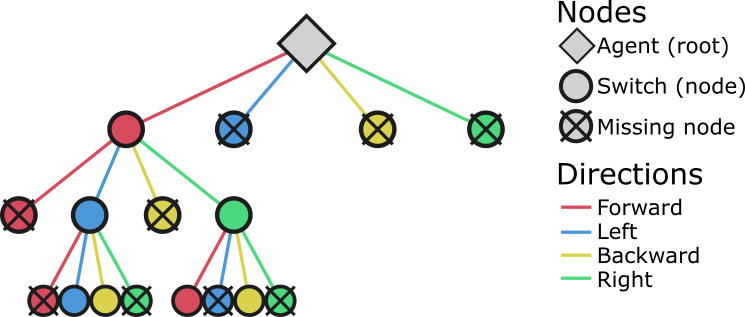
\includegraphics[height=0.3\textwidth]{assets/environment/treeobs.png}
        \caption*{Default Flatland \alert{Tree Observator}}
    \end{figure}
\end{frame}

%%%
\begin{frame}{Search Strategy}
    We preferred the \textbf{breath first} strategy with respect to the depth first strategy previously adopted for branch exploration.
    
    Flatland switches often create railways which immediately merge again with the previous one. Those are really useful to avoid collision and traffic, but on the other hand we will have nodes explored twice during observation. 
\end{frame}
%branches%%
\begin{frame}{Explored Branches}
    Considering that in \alert{straightaways}:
    \begin{itemize}
        \item It's not optimal for a train to stop
        \item Actions \texttt{LEFT} and \texttt{RIGHT} do not matter
    \end{itemize}
    We have improved the environment by \emph{requiring an action} only when a train is:
    \begin{itemize}
        \item At an intersection, allowing the choice of \textbf{direction}
        \item Approaching an intersection, allowing the choice of \textbf{stopping}
    \end{itemize}    
\end{frame}

%%%
\begin{frame}{Explored Branches}
    Flatland switches allow \alert{only two} possible directions and, as already set in the default tree observator, we save only nodes corresponding to switches. 
    
    \vspace{0.5cm}
    \begin{columns}
        \column{0.4\textwidth}
            The result of the observation is then a \textbf{binary tree}: only the leftward and the rightward child are created.
        
        \column{0.5\textwidth}
        \begin{figure}
            \centering
            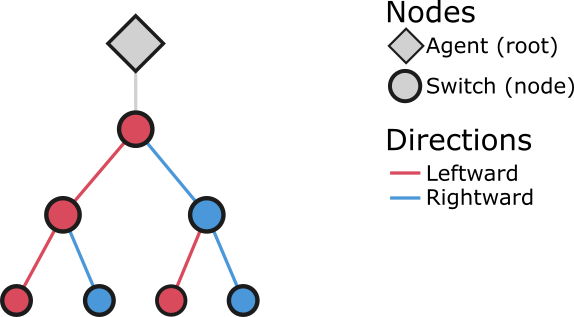
\includegraphics[width=1\textwidth]{assets/environment/binaryobs.png}
        \end{figure}
            
    \end{columns}
\end{frame}

%%%
\begin{frame}{Actions}
    We defined an \alert{Environment Wrapper} that requires trains to provide actions only in proximity of rail switches:
    \begin{figure}
        \centering
        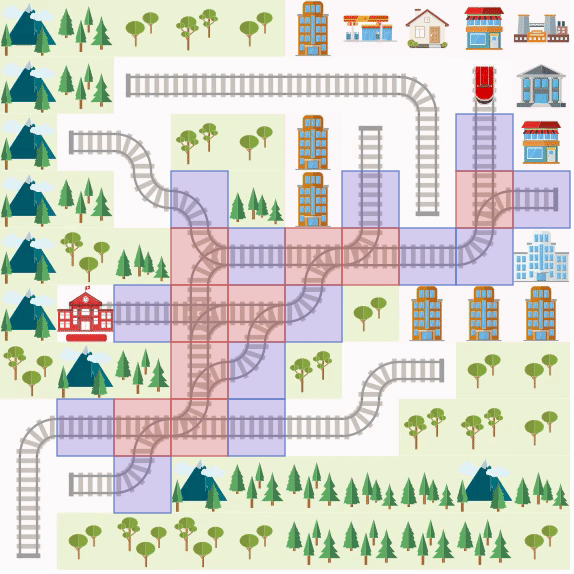
\includegraphics[width=0.45\textwidth]{assets/environment/switch_highlights.png}
        \captionsetup{justification=centering}
        \caption*{Railway sections where the train action is required. \\ \textcolor{Bittersweet}{In red: switches}\\ 
        \textcolor{NavyBlue}{In blue: tiles before or after a switch}}
        \label{fig:my_label}
    \end{figure}
\end{frame}


%%%
\begin{frame}{Actions}
    Considering the flatland environment, we have also optimized the set of possible actions, limiting them into: \texttt{STOP, MOVE LEFTWARD, MOVE RIGHTWARD}:
    \begin{figure}
        \centering
        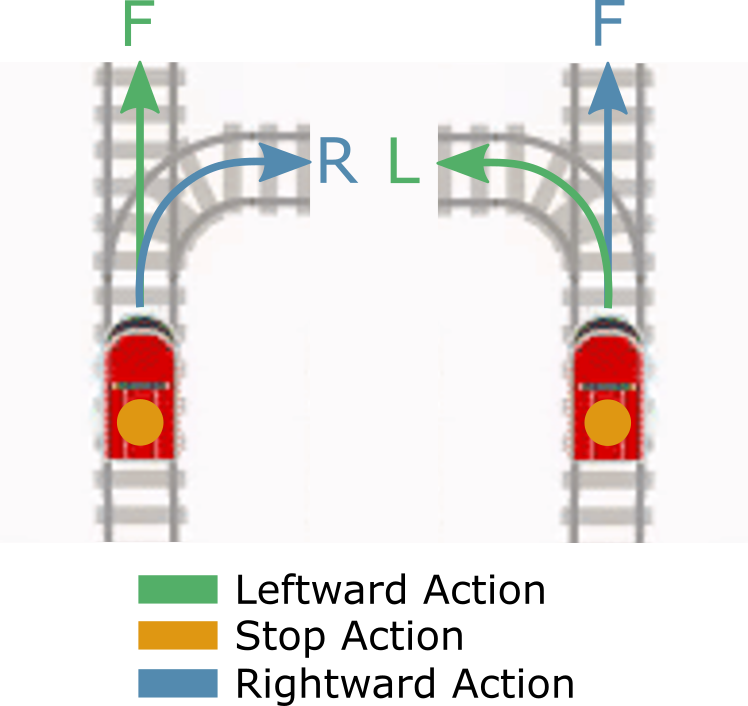
\includegraphics[width=0.4\textwidth]{assets/environment/actions.png}
        \caption*{Example of \alert{custom actions}, remapped to the Flatland's actions \texttt{(Left, Forward, Right, Stop)}}
    \end{figure}
\end{frame}

%%%
\begin{frame}{Reward}
    The flatland default reward is not enough to determine if a path could be a good one or not.
    
    Therefore we introduced a positive and a negative reward. We call them \textbf{attractive force} and \textbf{repulsive force} because they refer to gravitational force. The first represents the attraction towards the target, while the second represents the repulsion from agents moving in opposite direction.
    \begin{align*}
        force_{attractive} &= \frac{MASS_{TARGET}}{dist^2} \\
        force_{repulsive} &= \sum \frac{MASS_{AGENT} * N_{OPPOSITE AGENTS}}{dist^2}
    \end{align*}
\end{frame}


% =================================================================
% ==================== REINFORCEMENT LEARNING =====================
% =================================================================


\section{Reinforcement Learning}
%%% 
\begin{frame}{Reinforcement Learning}
    Reinforcement Learning is a technique in which
    \alert{agents} interacting with an \alert{environment}, learn the best \alert{actions} given the \alert{observations} from the environment, by \textit{maximizing} a \alert{reward function}. 
    \vspace{0.5cm}
    \begin{columns}
        \column{0.6\textwidth}

        \textbf{Execution of a RL step:}
        \begin{enumerate}
            \item Agent \textbf{observes} the environment
            \item Agents chooses an \textbf{action}
            \item Environment executes the action, advancing its \textbf{state}
            \item A \textbf{reward} is provided to the agent, which is then used by the \textbf{RL Algorithm} to learn the best action
        \end{enumerate}
        \column{0.4\textwidth}
        \begin{figure}
            \centering
            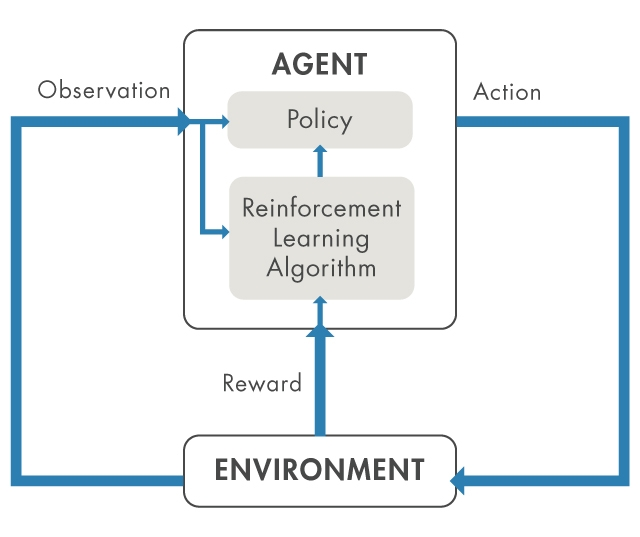
\includegraphics[width=1\textwidth]{assets/rl/rl.png}
        \end{figure}
    \end{columns}
\end{frame}

%%%
\begin{frame}{Q-Learning}
    The most simple RL algorithm is \alert{Q-Learning}. It uses:
    \begin{itemize}
        \item A \alert{Q-Table} that maps \textit{state-action} pairs into numeric "quality" values 
        \[Q: S \times A \to \mathbb{R}\]
        \item \alert{Temporal Difference Learning}, that accounts for the delayed future rewards as an effect of an action
        \[Q^{new}(s_t, a_t) \leftarrow Q(s_t, a_t) + \alpha \cdot [r_t + \gamma \cdot \max_a{ Q(s_{t+1}, a_t)} - Q(s_t, a_t)] \]
        where
        \begin{itemize}
            \item $s_t, a_t, r_t$ are the state, action and reward in the timestep $t$
            \item $\alpha$ is the \textit{learning rate}
            \item $\gamma$ is the \textit{discount factor}
        \end{itemize}
    \end{itemize}
\end{frame}

%%%
\begin{frame}{Deep-Q-Learning}
    Since traditional Q-Learning uses a table, it quickly becomes unfeasible as the observation space and action space increases. To solve this, \textbf{neural networks} are used to \textit{approximate} the Q-Table.
    
    The networks, instead of mapping state-action pairs into a single Q-Value, map states to \textbf{multiple Q-Values}, one for each action.
    
    \begin{figure}
        \centering
        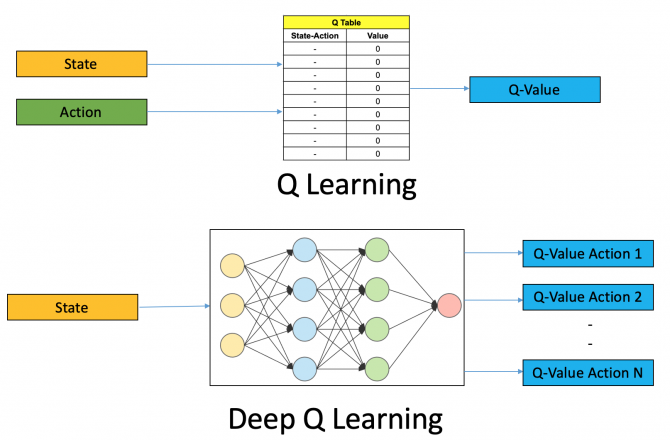
\includegraphics[width=0.5\textwidth]{assets/rl/q-vs-dqn.png}
    \end{figure}
\end{frame}

%%%
\begin{frame}{Deep-Q-Learning}
To train the network, the \alert{loss} function is defined as the \textit{distance from the expected Q-Value and the prediction}:
\[L(\theta) = (\mathbb{E}_{s'}[r + \gamma \max_{a'}{Q(s',a')]} - Q(s,a,\theta))^2 \]

The loss is computed using an \alert{experience memory} that contains $(s_i, a_i, r_i, s_{i+1})$ tuples. 
%This memory can be:
%\begin{itemize}
%    \item Sampled \textbf{randomly}
%    \item Sampled prioritizing \textbf{recent} entries
%    \item Sampled prioritizing entries that have higher \textbf{losses}
%\end{itemize}

In this project the experiences stored inside the memory are sampled \textbf{randomly} with an uniform distribution.
\end{frame}

%%%
\begin{frame}{Double Deep-Q-Learning}
    A variant of DQN, called \alert{Double Deep Q-Learning} that reduces \textbf{bias overestimation} by:
    \begin{itemize}
        \item Using \textbf{two neural networks} with parameters $\theta$ and $\theta'$, alternating their roles
        \item A loss function using the second network to estimate the expected Q-Value
        \[L(\theta) = (\mathbb{E}_{s'}[r + \gamma Q(s', \overline{a} | \theta')] - Q(s', a' |\theta))^2\]
        \[\overline{a} = \arg\max_{a'}{Q(s',a' | \theta)}\]
        \item Periodically updating the first network with the parameters of the second, either with a full overwrite (hard update) or a weighted mean (soft update)
    \end{itemize}
\end{frame}

% =================================================================
% ====================       POLICIES         =====================
% =================================================================


%%%
\begin{frame}{Policies}
    \alert{Policies} are functions $\pi(a | s)$ that determine which actions to choose in a given state.
    \begin{itemize}
        \item \textbf{In testing} the action associated to the best Q-Value is always chosen
        \item \textbf{In training} the actions are chosen with a random probability, to explore novel strategies
    \end{itemize}
\end{frame}

%%%
\begin{frame}{Policies}
    We used three policies to test their performance in training speed:
    \begin{itemize}
        \item \alert{Epsilon Greedy Policy}: selects a random with probability $\epsilon$, otherwise the best action currently learnt
        \item \alert{Softmax}: the Q-Values are normalized using the softmax-function and used as probabilities to select the action
        \item \alert{Boltzmann}: a variation of softmax, which uses an hyper-parameter called \textit{temperature} $\tau$ to modify the distribution. 
        \begin{itemize}
            \item Higher $\tau \ \to$ more deviation (more spread)
            \item Lower $\tau \ \to$ less deviation (higher peaks)
        \end{itemize}
    \end{itemize}
\end{frame}

%%%
\begin{frame}{Policies}
    \begin{block}{\centering Epsilon Greedy}
    \centering
    \resizebox{0.5\textwidth}{!}{\begin{tikzpicture}[scale=0.8]
    \begin{axis}[
        mbarplot,
        bar width=1cm,
        ytick={1, 9},
        yticklabels={$\epsilon$, $1-\epsilon$},
        ylabel style={at={(0,0.5)}},
        ybar=-1cm,
        ymin=0, ymax=10,
        xtick={1, 2},
        xticklabels={Random, Best},
        xmin=0, xmax=3,
        grid=none,
        ylabel={Probability},
    ] 

    \addplot plot coordinates {(1,1)};
    \addplot plot coordinates {(2,9)};
    \addplot[black,dotted, sharp plot,update limits=false,] coordinates {(0.1,1) (0.8,1) };
    \addplot[black,dotted, sharp plot,update limits=false,] coordinates {(0.1,9) (1.8,9) };

    \end{axis}
\end{tikzpicture}
}
    \[a = \begin{cases}
            \text{random action} & \text{if  } r < \epsilon  \\
            \arg\max_a \ Q(s, a) & \text{if  } r \geq \epsilon
           \end{cases}
    \]
    \end{block}
\end{frame}

%%%
\begin{frame}{Policies}
    \begin{columns}
        \column{0.5\textwidth}
        \begin{block}{\centering Softmax}
        \centering
        \resizebox{0.9\textwidth}{!}{\begin{tikzpicture}[scale=0.8]
    \begin{axis}[
        mbarplot,
        %ytick={1, 9},
        ylabel style={at={(0,0.5)}},
        %ybar=-1cm,
        ymin=0, ymax=1.3,
        xlabel={Action},
        xtick={0, 1, 2},
        xmin=-1, xmax=3,
        grid=none,
        area legend,
        legend columns=-1,
    ] 

    \addplot plot coordinates {(0, 0.42) (1, 1) (2, 0.28)};
    \addplot plot coordinates {(0, 0.27) (1, 0.49) (2, 0.24)};
    \legend{Action Q-Values, Action Probability}
    \end{axis}
\end{tikzpicture}
}
        \[ P(a_i) = \frac{e^{Q(s, a_i)}}{\sum_a e^{Q(s, a)}}\]
        \end{block}
        
        \column{0.5\textwidth}
        \begin{block}{\centering Boltzmann}
        \centering
        \resizebox{1\textwidth}{!}{\begin{tikzpicture}[scale=0.8]
    \begin{axis}[
        mlineplot,
        %ytick={1, 9},
        ylabel style={at={(0,0.5)}},
        %ybar=-1cm,
        ymin=0, ymax=1,
        xlabel={Action},
        xtick={0, 1, 2},
        xmin=-0.2, xmax=2.2,
        grid=none,
        %area legend,
        legend columns=1,
        legend style={anchor=north, at={(0.9,1)}},
    ] 
    \addplot plot [smooth] coordinates {(0, 0.42) (1, 1) (2, 0.28)};
    % t = 2
    \addplot plot [smooth] coordinates {(0, 0.32) (1, 0.4) (2, 0.28)};
    % t = 1
    \addplot plot [smooth] coordinates {(0, 0.27) (1, 0.49) (2, 0.24)};
    % t = 0.5
    \addplot plot [smooth] coordinates {(0, 0.20) (1, 0.65) (2, 0.15)};
    % t = 0.2
    \addplot plot [smooth] coordinates {(0, 0.05) (1, 0.93) (2, 0.026)};
    
    \legend{Action Q-Values, P(a) $\tau = 2$, P(a) $\tau = 1$, P(a) $\tau = 0.5$, P(a) $\tau = 0.2$}
    \end{axis}
\end{tikzpicture}
}
        \[ P(a_i) = \frac{e^{Q(s, a_i) / \tau}}{\sum_a e^{Q(s, a)/\tau}}\]
        \end{block}
    \end{columns}    
\end{frame}


% ==========================================================
% ==================== NEURAL NETWORKS =====================
% ==========================================================


\section{Neural Networks}
%%%
\begin{frame}{Sequential}
    In the project, all neural networks use a \alert{Sequential} (Feed Forward) architecture.
    
    Three networks were designed, each with its own characteristics, to compare their performance:
    
    \vspace{0.5cm}
    \centering
    \begin{tabular}{ccc}
        \toprule
        \textbf{Network} & \textbf{Parameters} & \textbf{Main Feature} \\
        \midrule
        seq1  & 288,003 & Dense layers \\
        seq2  & 128,387 & Dense layers \\
        conv1 & 7,551 &  Conv1D preprocessor + Dense layers\\
        \bottomrule
    \end{tabular}
\end{frame}

%%%
\begin{frame}{Dense}
    \begin{columns}
        \column{0.5\textwidth}
        \begin{figure}
            \centering
            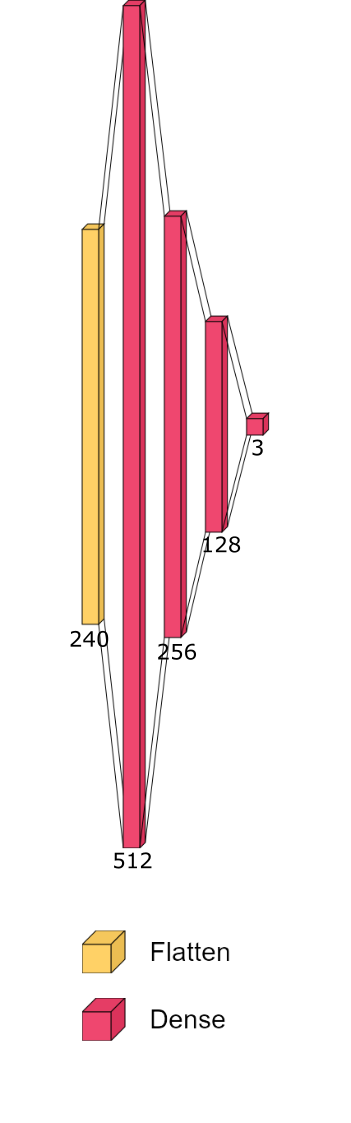
\includegraphics[height=1.2\textwidth]{assets/nets/seq1.png}
            \caption*{The \alert{\texttt{seq1}} network structure}
        \end{figure}
        
        \column{0.5\textwidth}
        \begin{figure}
            \centering
            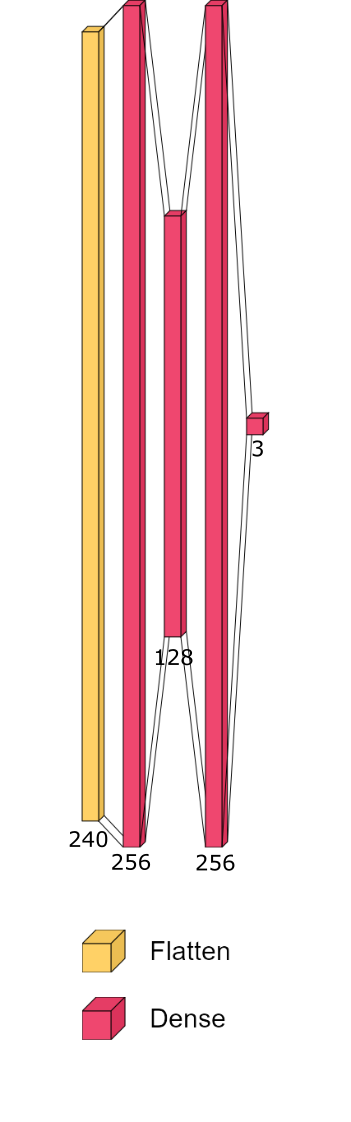
\includegraphics[height=1.2\textwidth]{assets/nets/seq2.png}
            \caption*{The \alert{\texttt{seq2}} network structure}
        \end{figure}
    \end{columns}
    
\end{frame}

%%%
\begin{frame}{Convolutional 1D}
    \begin{figure}
    \centering
    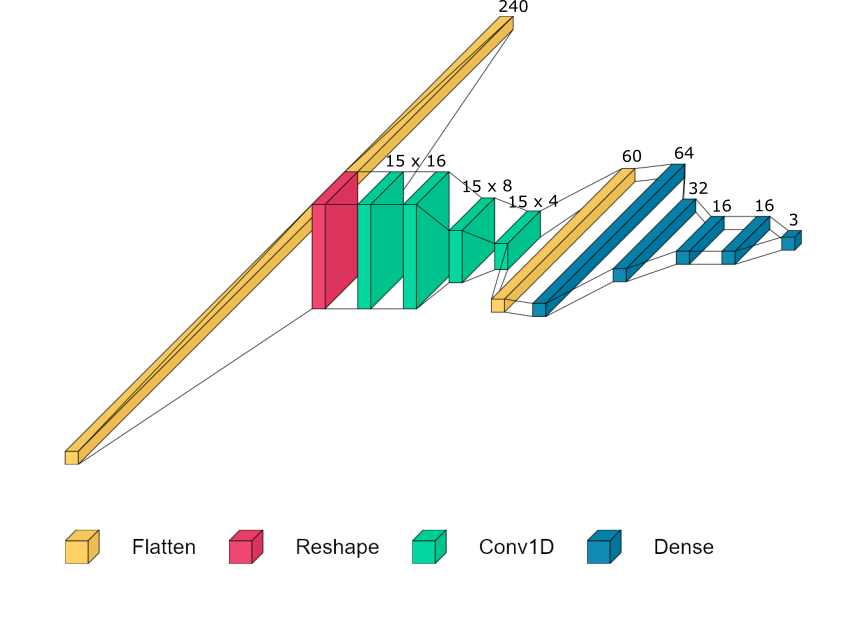
\includegraphics[width=0.8\textwidth]{assets/nets/conv1.png}
    \caption*{The \alert{\texttt{conv1}} network structure}
    \end{figure}
\end{frame}


%%%
\begin{frame}{Convolutional 1D}
    The main characteristics of the \alert{conv1} network are:
    \begin{itemize}
        \item The input is reshaped into a 15x16 matrix
        \item A series of 1D convolutional layers is used as a \alert{Preprocessor} to reduce the dimension of the observation
        \item The reduced observations, representing the "quality" of the network, are then used by a sequence of Dense layers to determine the final Q-Values
    \end{itemize}
    
    The advantage of this approach is a greatly reduced number of parameters, since the 1D convolution is parametrized only along one of its dimensions

\end{frame}

% =========================================================
% ==================== IMPLEMENTATION =====================
% =========================================================
\section{Implementation}

\begin{frame}{Frameworks}
    \begin{center}
    \begin{table}[h]
    \centering
    \begin{tabular}{|c|c|c|c|}
    \hline
    \ & Keras-RL & TF-Agents & Tensorforce \\
    \hline
    \ custom-env & \checkmark & \checkmark & \checkmark \\
    \ custom-actions & \checkmark & \checkmark & \checkmark \\
    \ custom-memory & \checkmark & - & - \\
    \ framework-based & - & \checkmark & \checkmark \\
    \ policies & \checkmark & \checkmark & - \\
    \ callbacks & \checkmark & - & - \\
    \ DQN & \checkmark & \checkmark & \checkmark \\
    \ DDQN & \checkmark & \checkmark & \checkmark \\
    \ DDQN (dueling) & \checkmark & - & \checkmark \\
    \ multi-actions & \checkmark & - & - \\
    \ multi-agents & - & - & - \\
    \hline
    \end{tabular}
    \end{table}
    \end{center}
\end{frame}


\begin{frame}{Keras-RL with Multi-Agent support}
    \begin{figure}
    \centering
    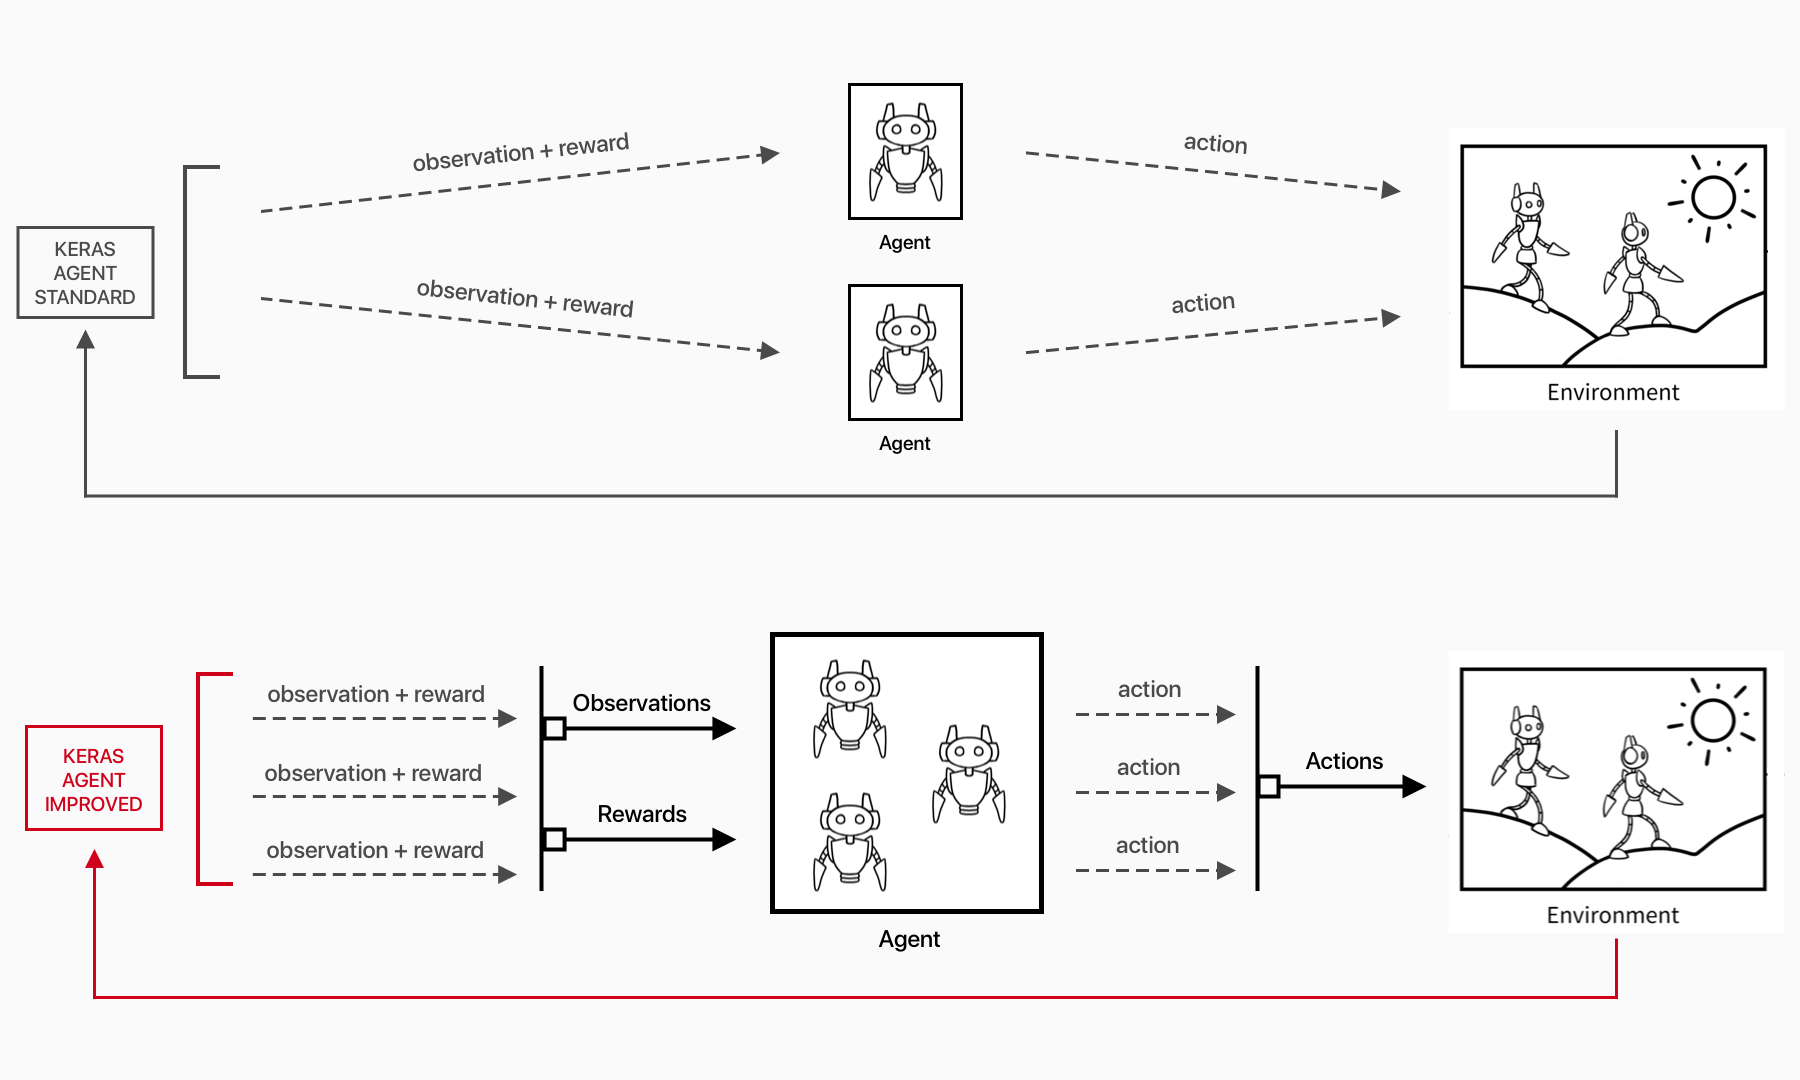
\includegraphics[width=1\textwidth, height=0.65\textwidth]{assets/rl/keras.png}
    \end{figure}
\end{frame}

% =================================================================
% ==================== RUNNING CONFIGURATIONS =====================
% =================================================================


\section{Configuration Of The Experiments}

\begin{frame}{Baseline and Builder}
    \begin{figure}
    \centering
    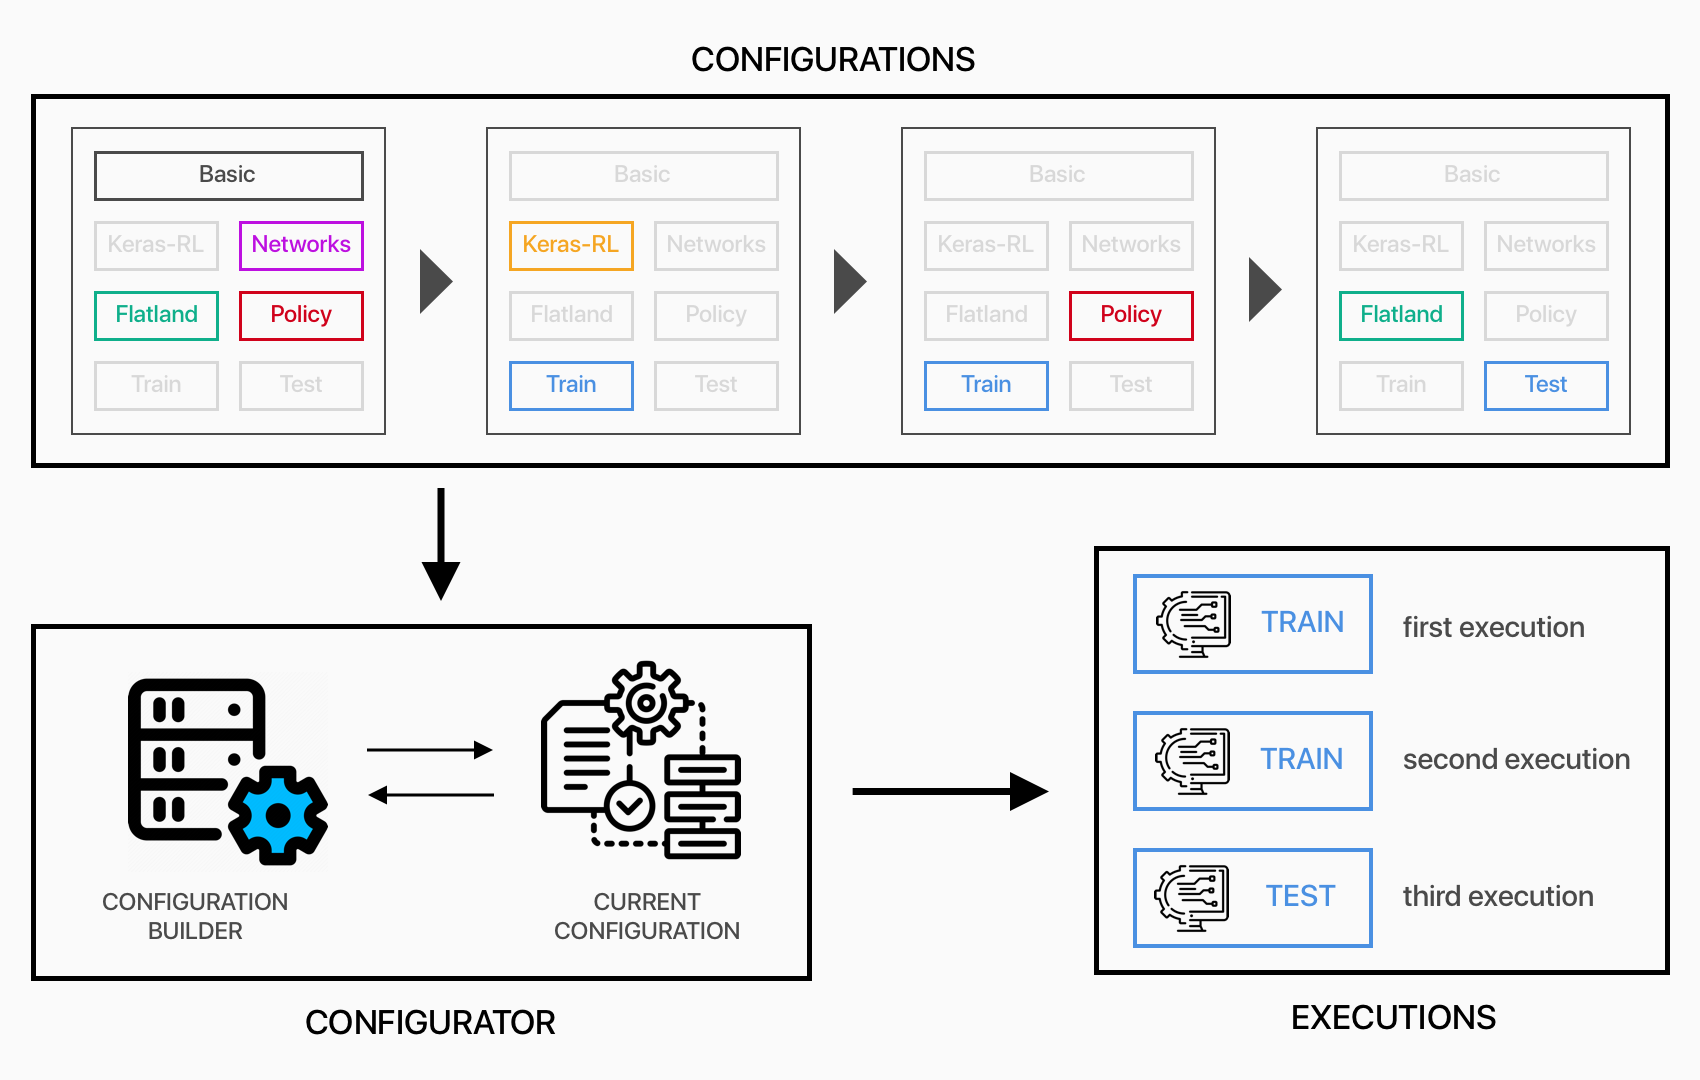
\includegraphics[width=1\textwidth]{assets/configs.png}
    \end{figure}
\end{frame}

\begin{frame}[fragile]{Flatland}
The static configuration of the \alert{Flatland} environment used inside all the training/testing experiments is:
\newline
\begin{lstlisting}[language=json,firstnumber=1]
{
    "map_width": 28,
    "map_height": 21,
    "n_cities": 2,
    "max_rails_in_city": 4,
    "max_rails_between_cities": 4,
    "cities_grid_distribution": false,
    "malfunction_rate": 0.0001,
    "malfunction_min_duration": 1,
    "malfunction_max_duration": 5
}
\end{lstlisting}
\end{frame}


% ==================================================
% ==================== RESULTS =====================
% ==================================================

\section{Analysis and Results}
%%%
{\setbeamercolor{background canvas}{bg=white}
\begin{frame}{Networks}
    Evaluation of the three network \textbf{topologies}: \alert{seq1}, \alert{seq2} and \alert{conv1}, on 100 episodes of maximum 500 steps each.
    
    \begin{columns}
        \column{0.5\textwidth}
        \begin{figure}
            \centering
            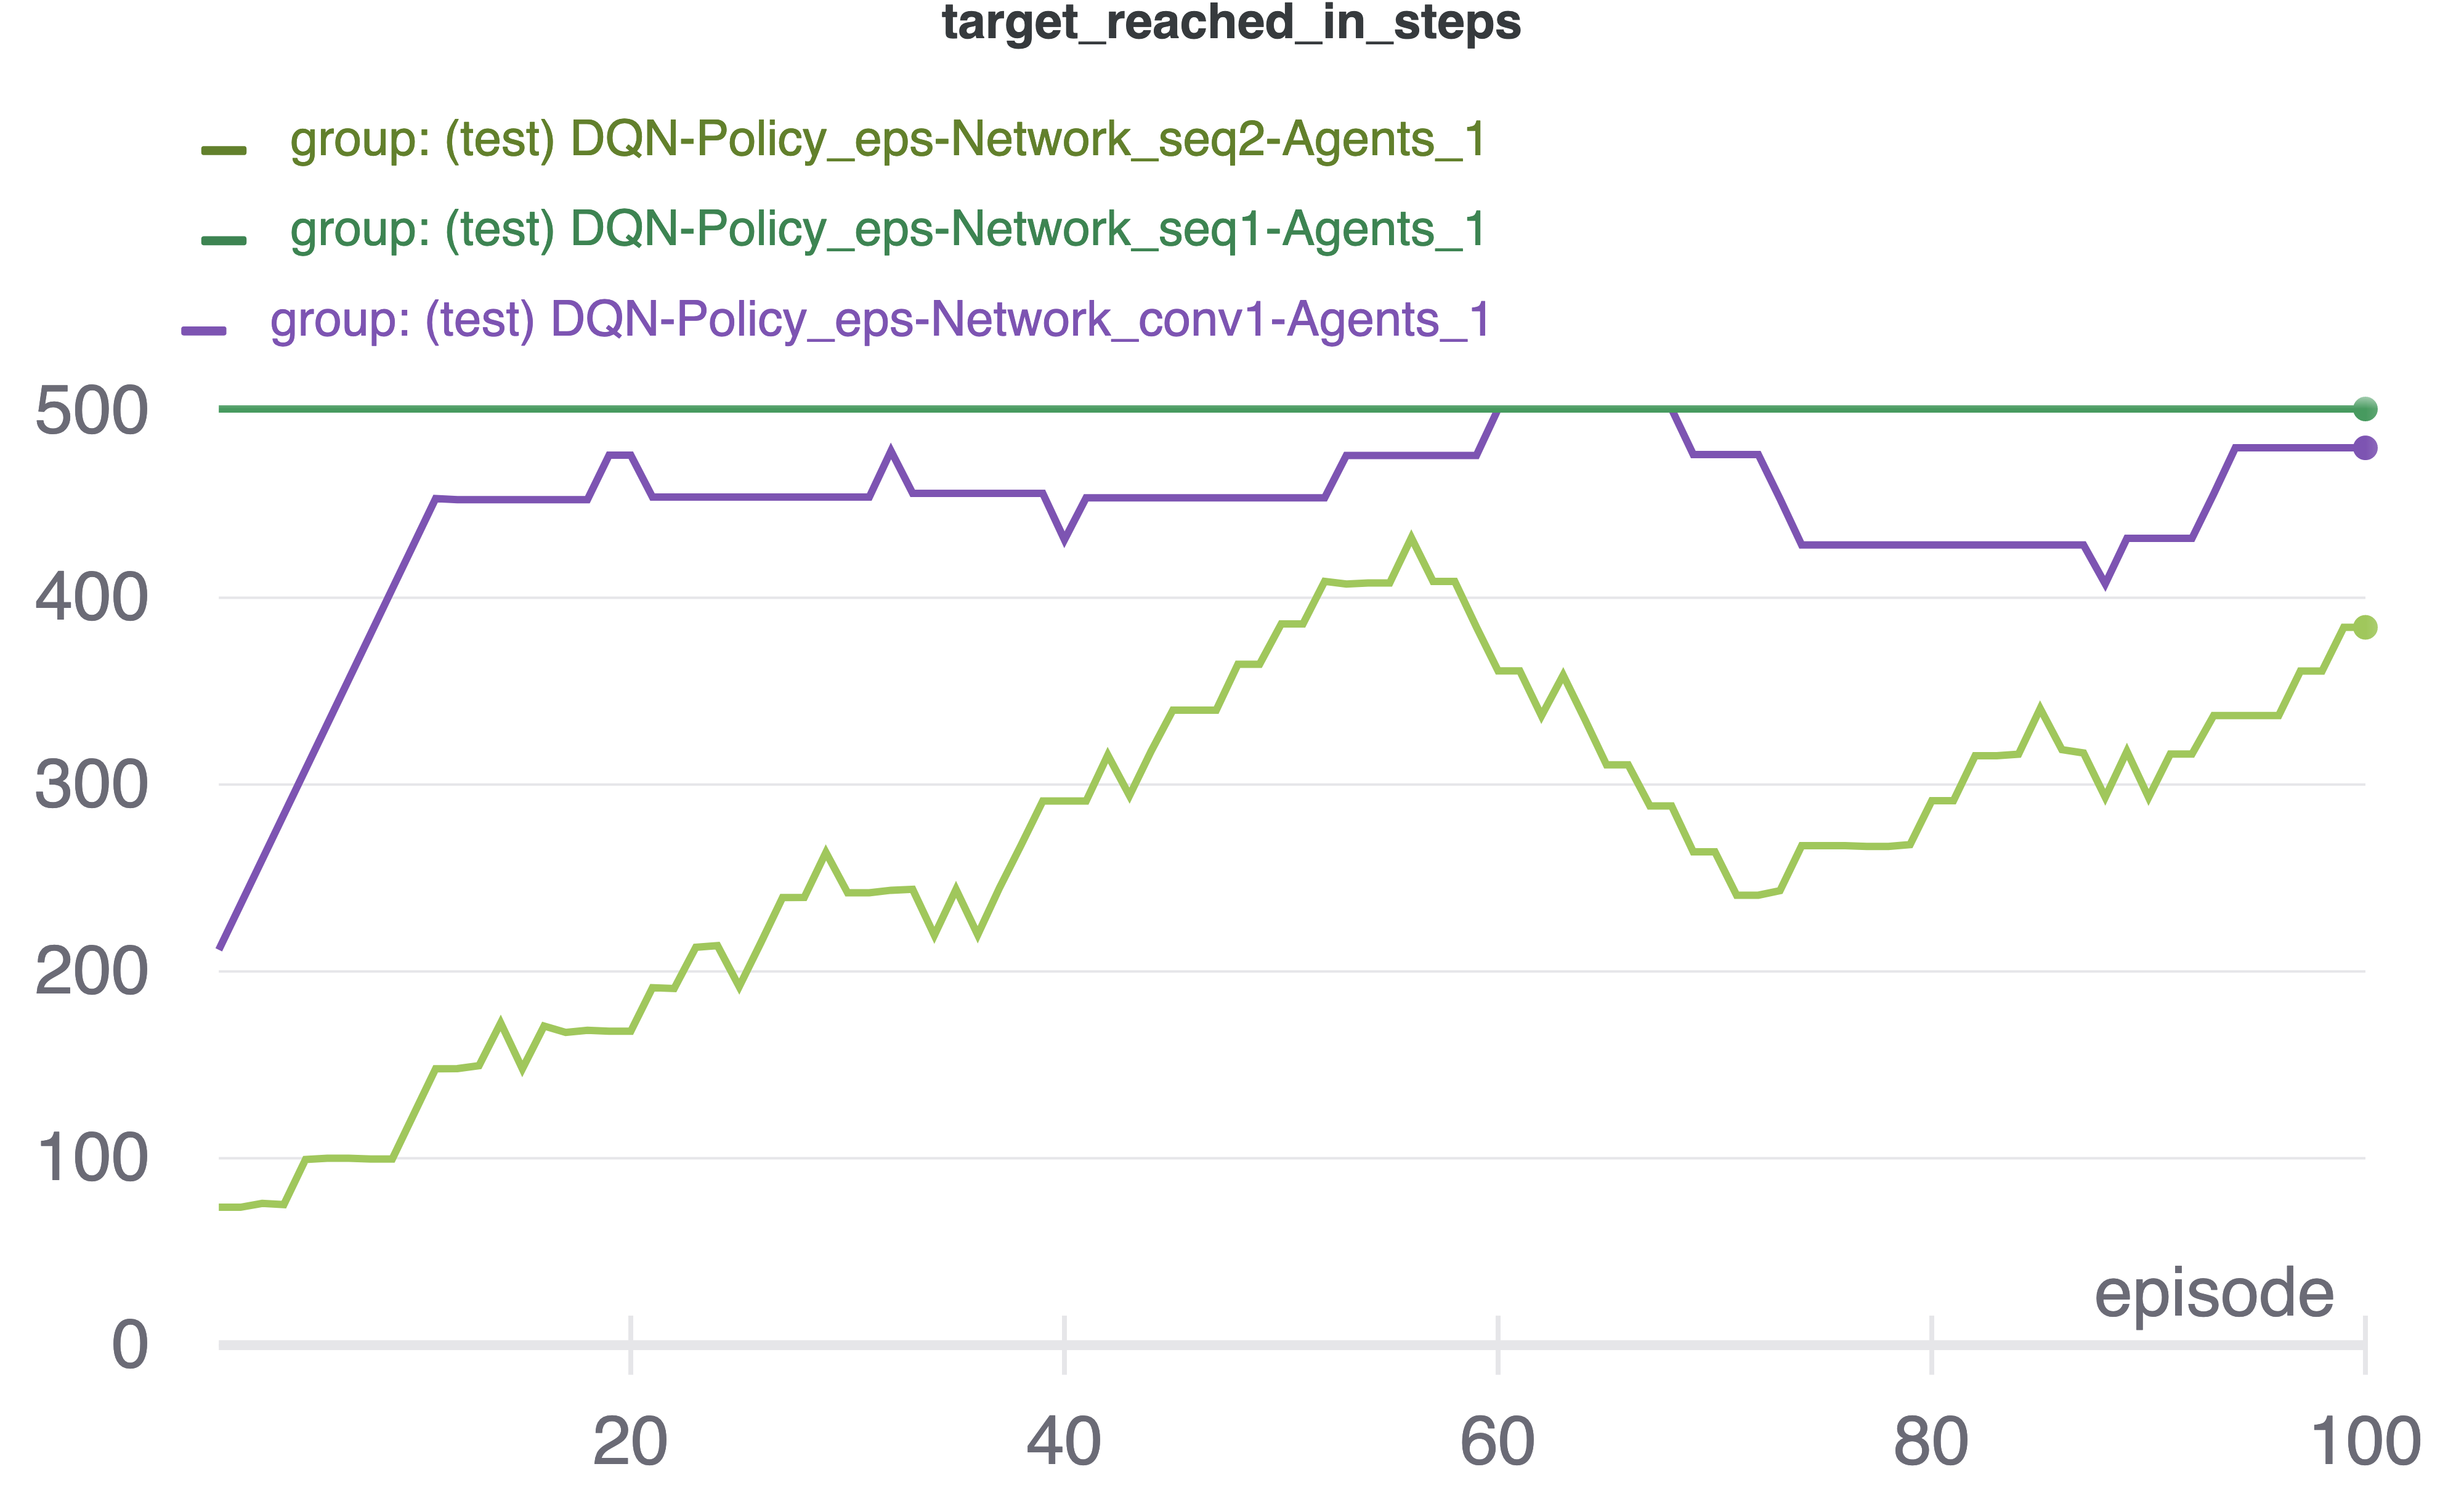
\includegraphics[width=1\textwidth, height=0.75\textwidth]{assets/results/nets/target_reached_in_steps.png}
            \caption*{Number of steps to reach the target}
        \end{figure}
        
        \column{0.5\textwidth}
        \begin{figure}
            \centering
            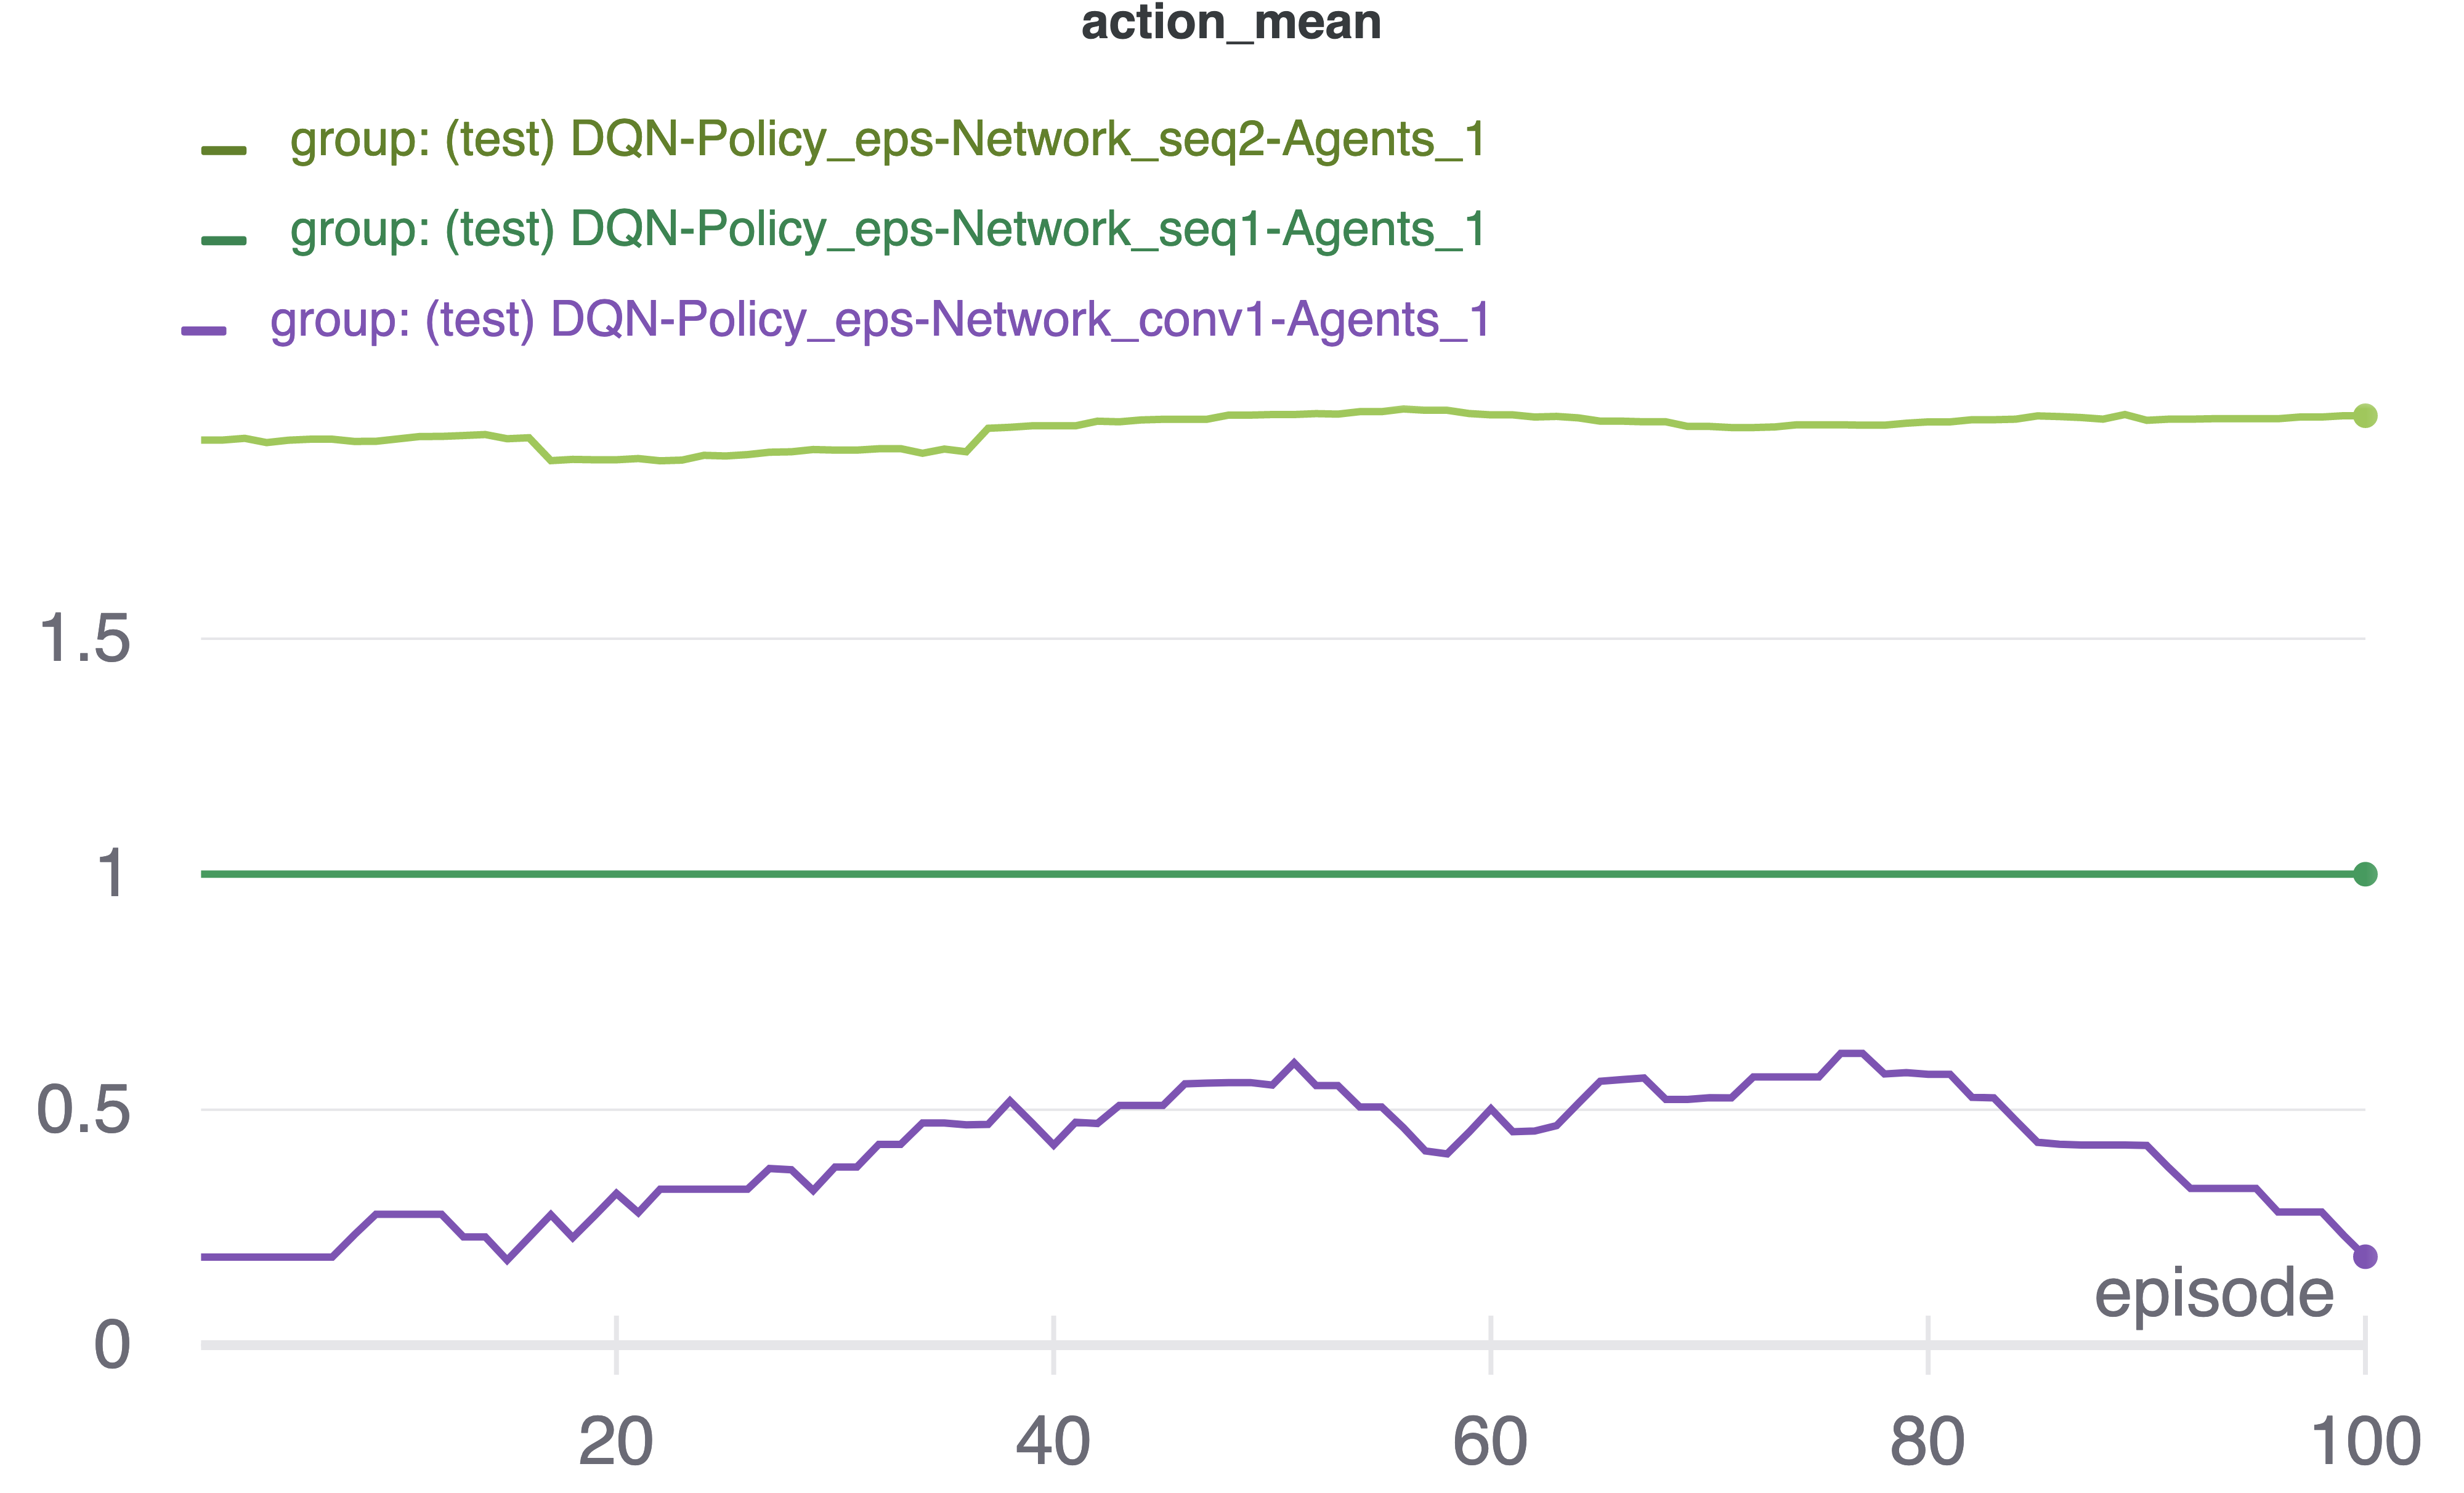
\includegraphics[width=1\textwidth, height=0.75\textwidth]{assets/results/nets/action_mean.png}
            \caption*{Mean action value}
        \end{figure}
    \end{columns}
\end{frame}
}

%%%
{\setbeamercolor{background canvas}{bg=white}
\begin{frame}{Policies}
    Training performance for the \textbf{policies}: \alert{Epsilon-Greedy} and \alert{Boltzmann}, using the \textit{seq2} network, carried out over 500,000 training steps
    \begin{figure}
        \centering
        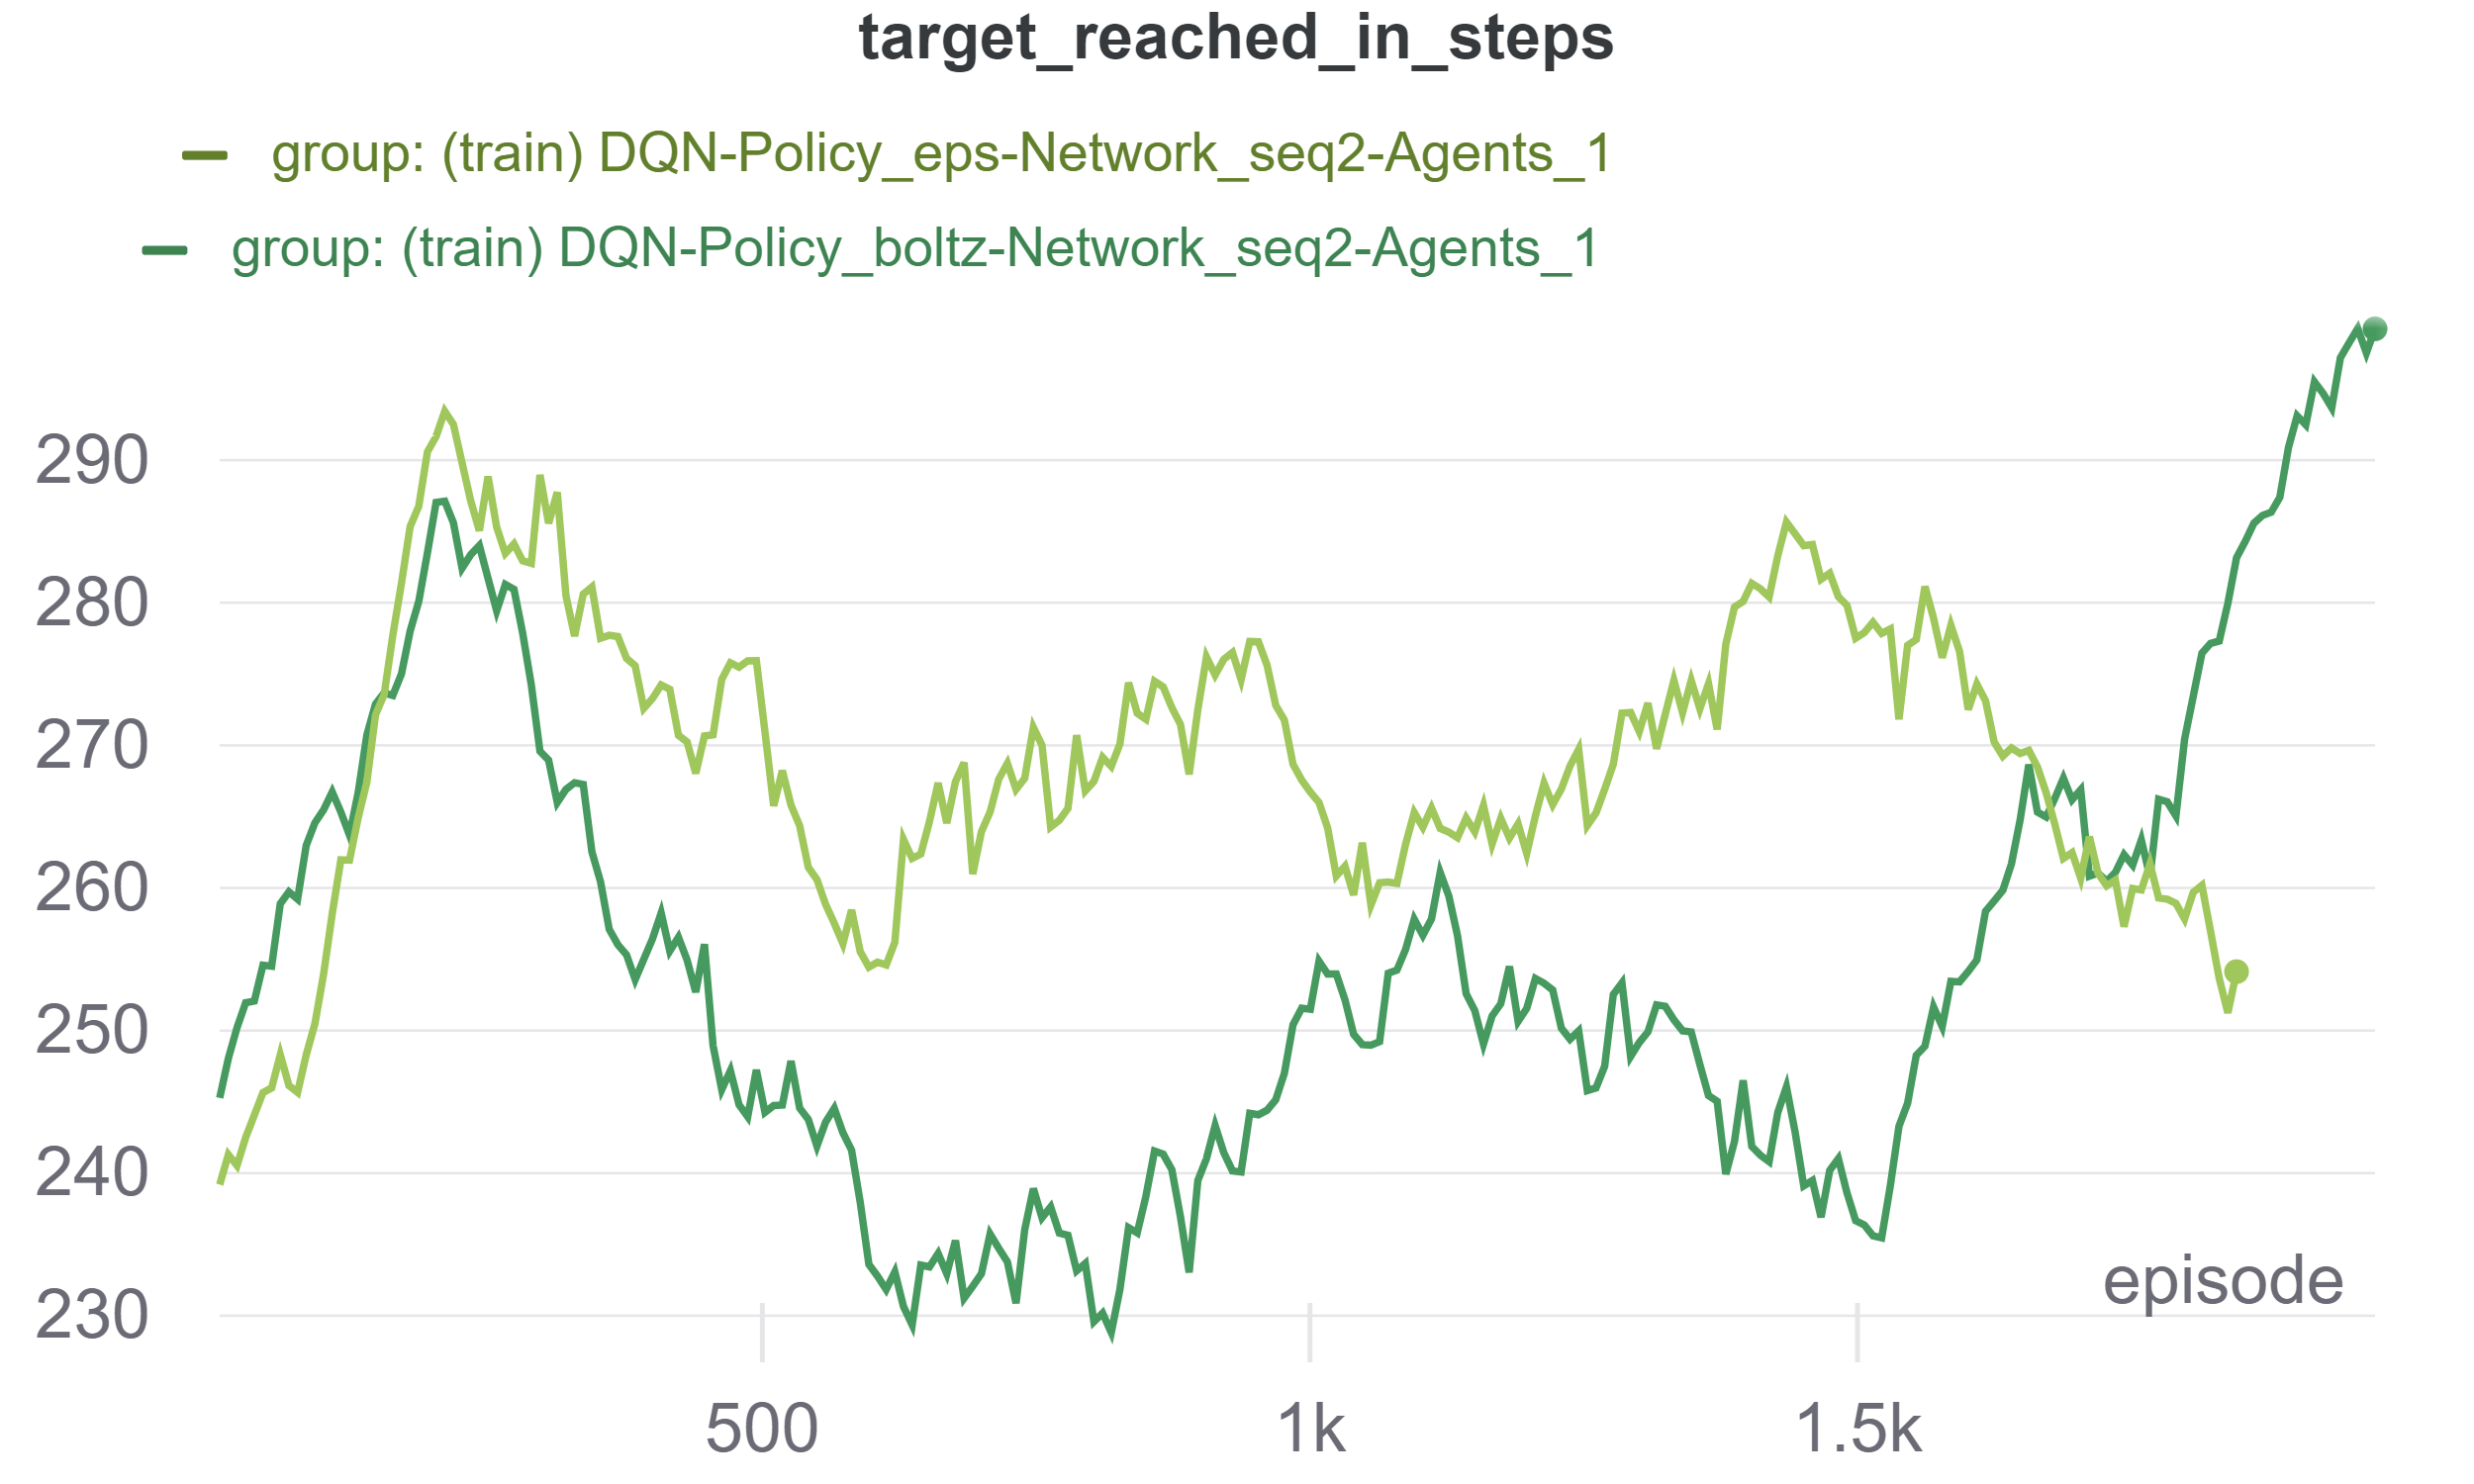
\includegraphics[width=0.5\textwidth, height=0.375\textwidth]{assets/results/policy/target_reached_in_steps.png}
        \caption*{Number of steps to reach the target}
    \end{figure}
\end{frame}
}

%%%
{\setbeamercolor{background canvas}{bg=white}
\begin{frame}{RL Algorithms}
    Training and testing performance of \alert{DQN} and \alert{DDQN}, using the \textit{seq2} network and \textit{boltzmann} policy. \\
    Training was carried out over 500,000 training steps and then tested on 100 episodes with 500 steps maximum each.
    
    \begin{columns}
    \column{0.5\textwidth}
    \begin{figure}
        \centering
        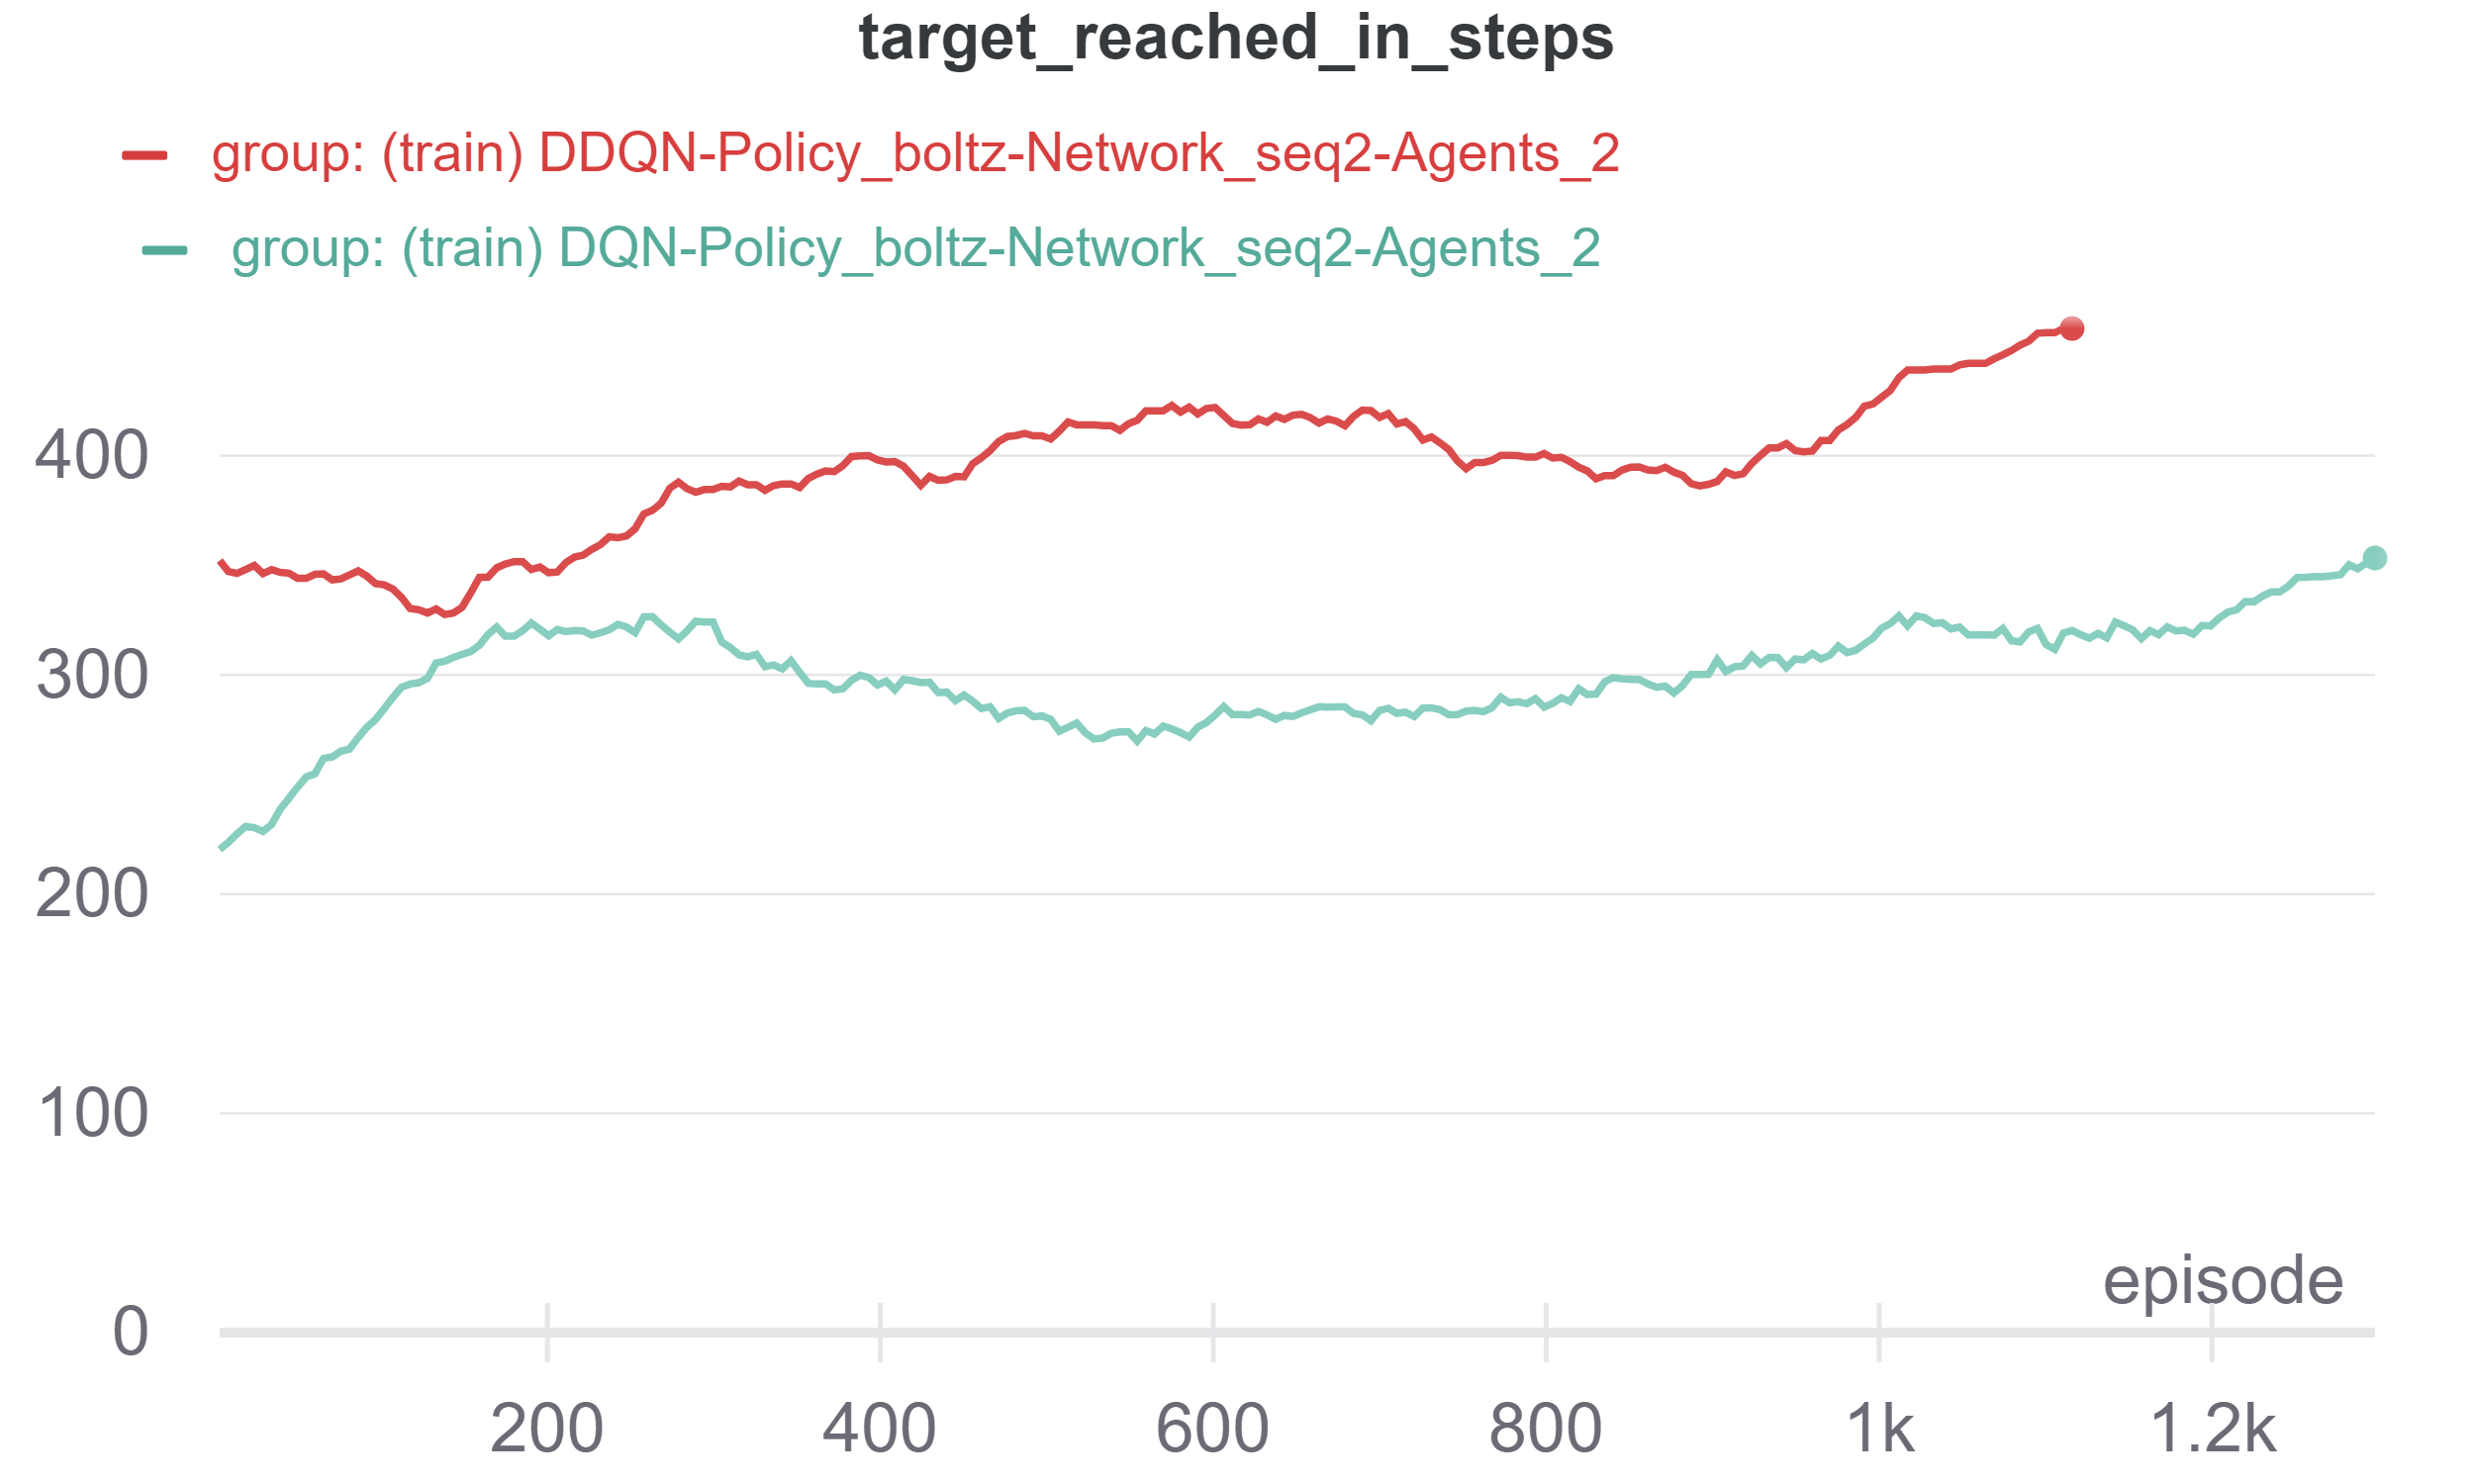
\includegraphics[width=1\textwidth, height=0.75\textwidth]{assets/results/rl/target_reached_in_steps.png}
        \caption*{\textbf{Training} - Number of steps to reach the target}
    \end{figure}
    \column{0.5\textwidth}
    \begin{figure}
        \centering
        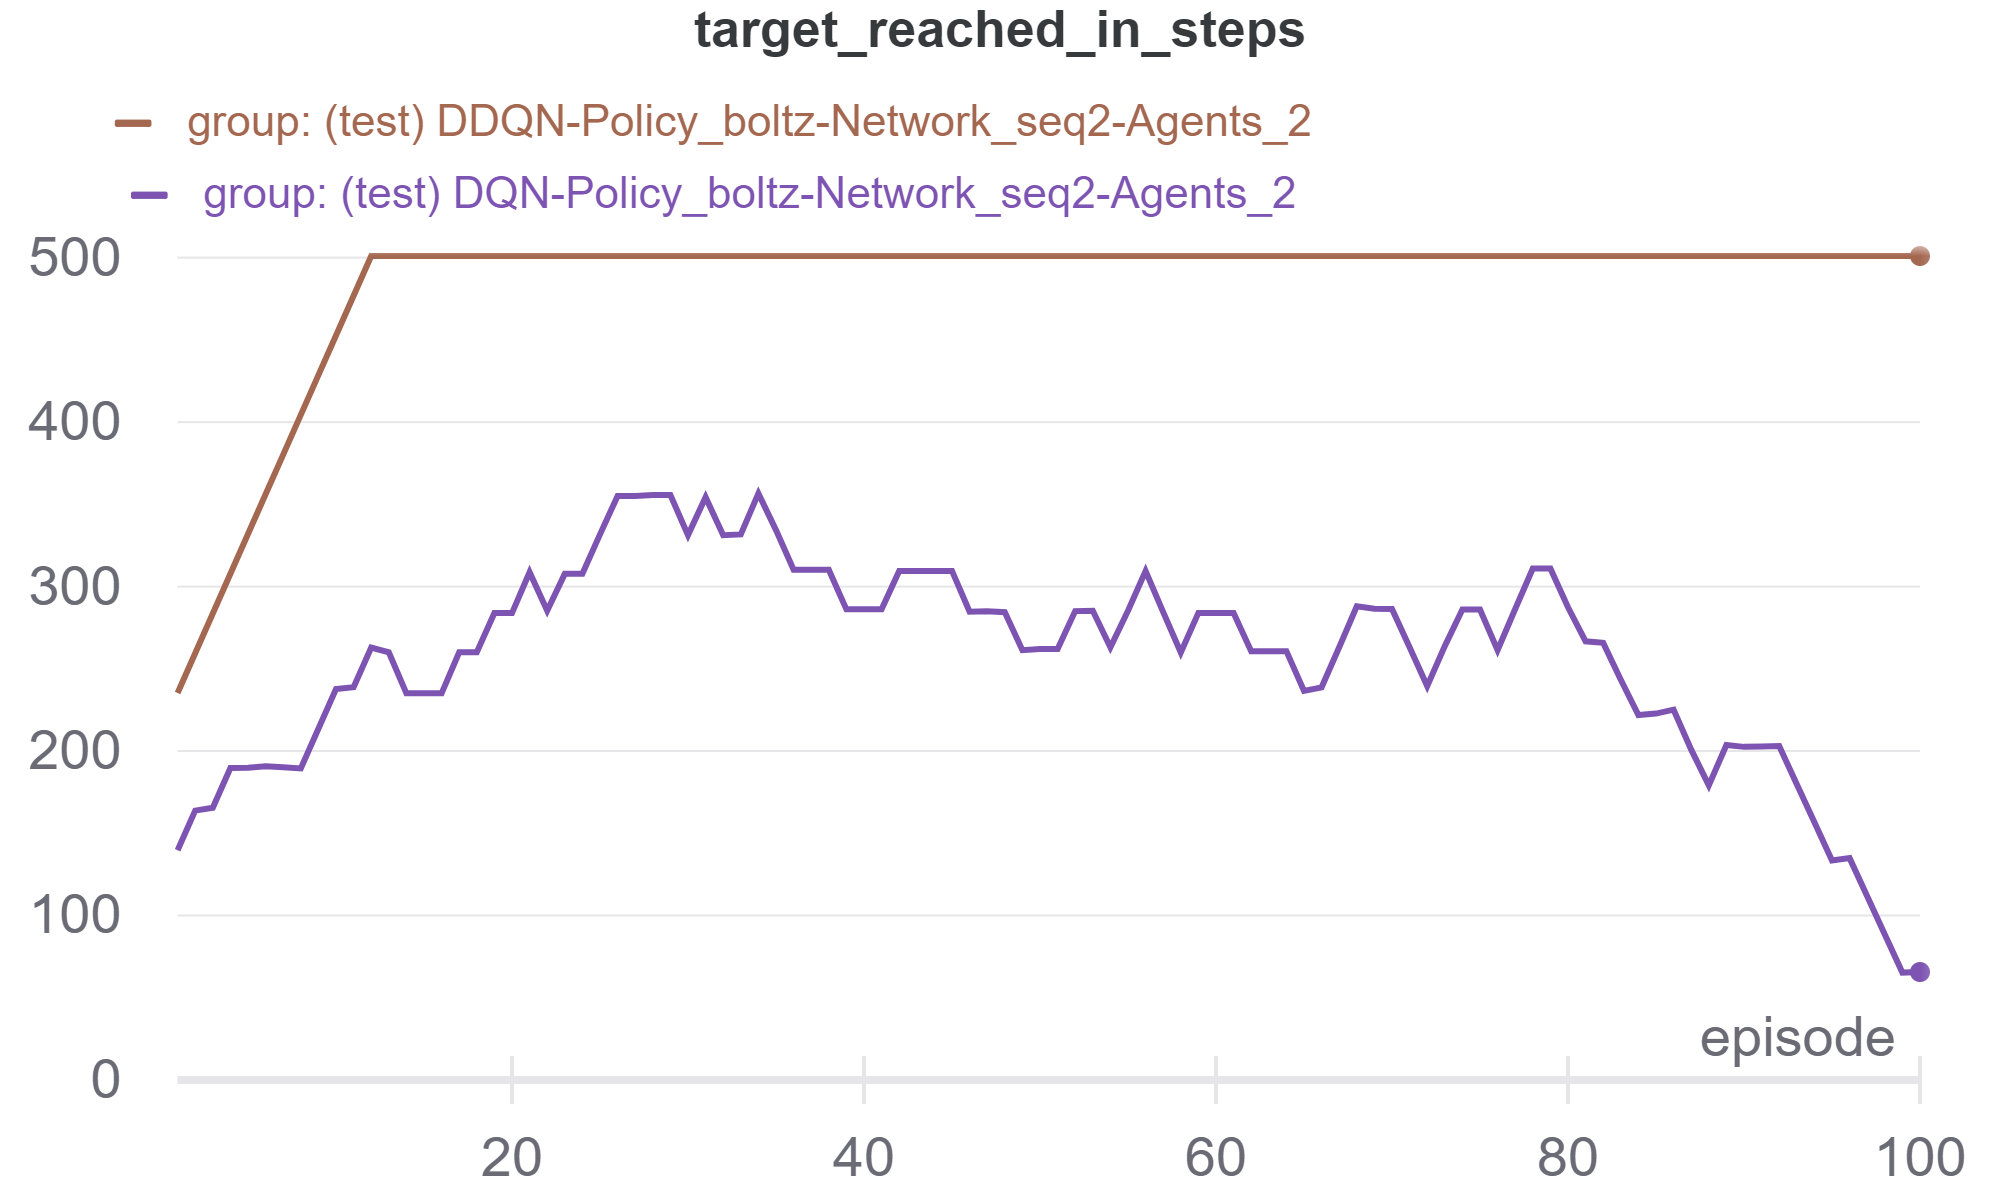
\includegraphics[width=1\textwidth, height=0.75\textwidth]{assets/results/rl/target_reached_in_steps_t.png}
        \caption*{\textbf{Testing} - Number of steps to reach the target}
    \end{figure}
    \end{columns}
\end{frame}
}

%%%
{\setbeamercolor{background canvas}{bg=white}
\begin{frame}{Agents}
    Finally, to evaluate the performance in the multi-agent environment, a \textbf{DQN} with \textbf{seq2} network and \textbf{boltzmann} policy was tested in environment with \alert{one}, \alert{two} and \alert{three agents}.\\
    Testing was carried out over 100 episodes, of 500 steps each.
    
    \begin{columns}
    \column{0.5\textwidth}
    \begin{figure}
        \centering
        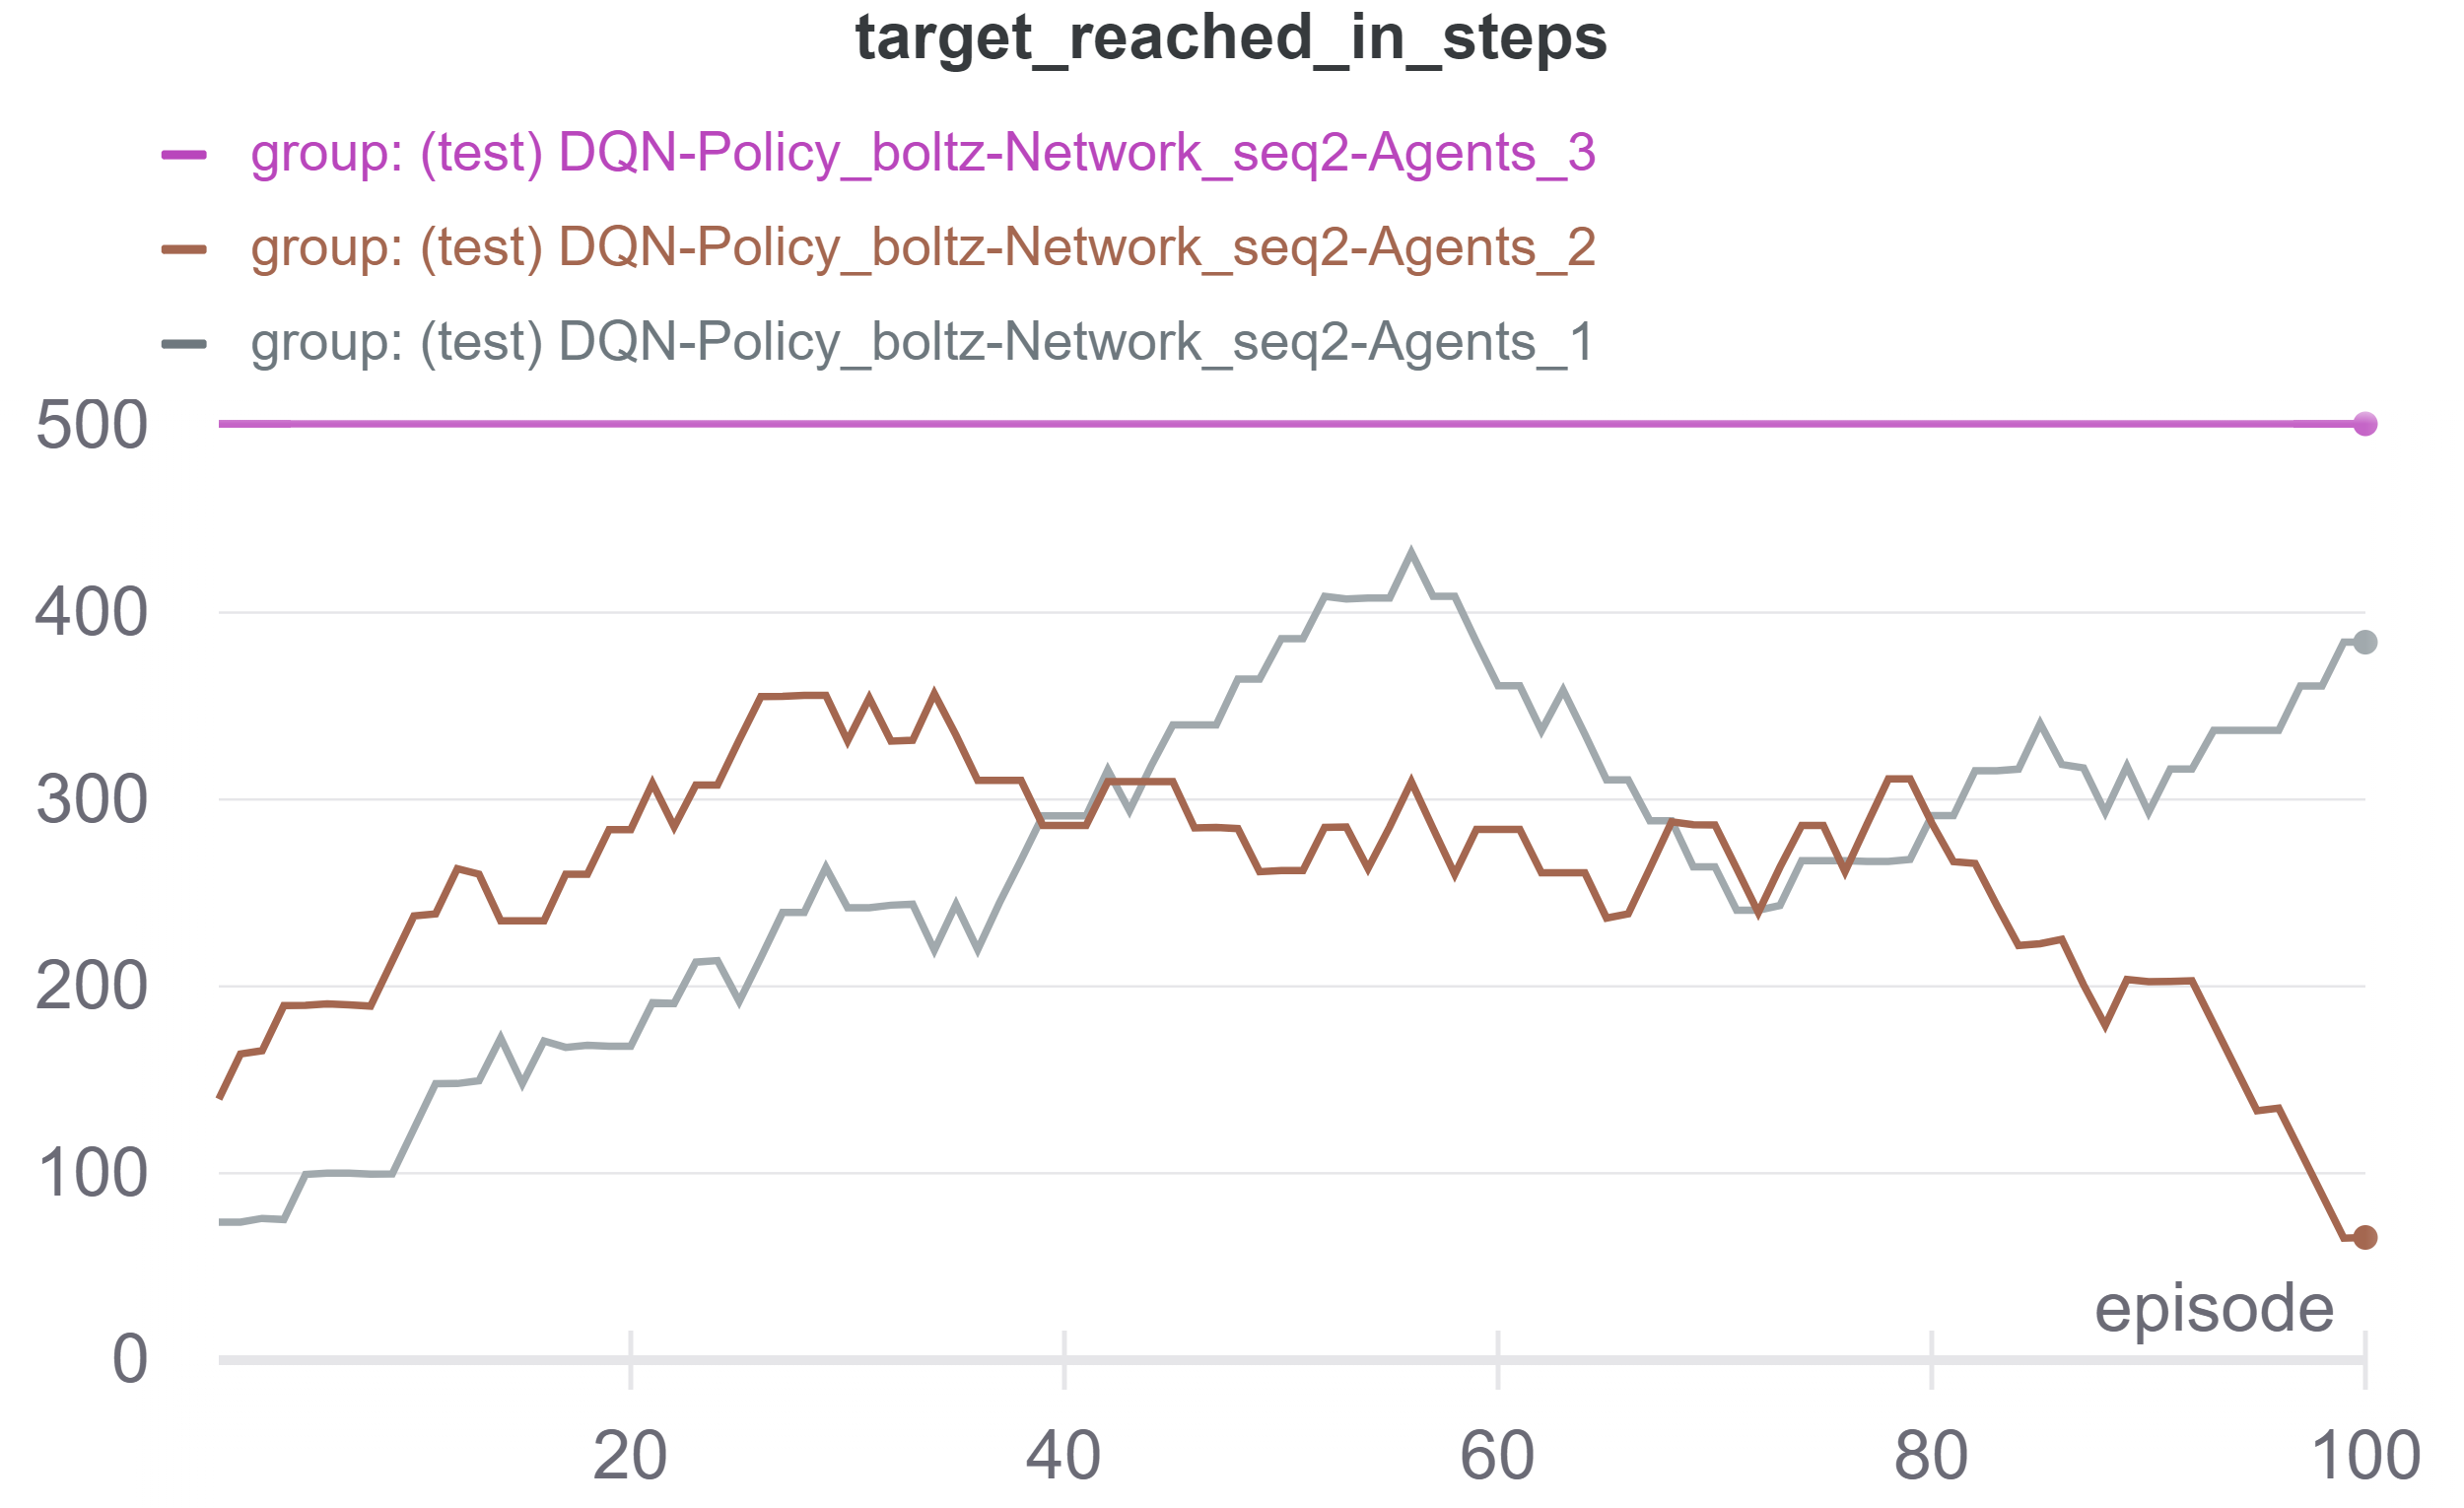
\includegraphics[width=1\textwidth, height=0.75\textwidth]{assets/results/agents/target_reached_in_steps.png}
        \caption*{Number of steps (for each agent) to reach their target}
    \end{figure}
    \column{0.5\textwidth}
    \vspace{-0.45cm}
    \begin{figure}
        \centering
        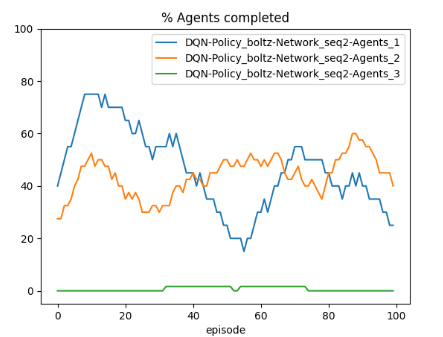
\includegraphics[width=1\textwidth, height=0.75\textwidth]{assets/results/agents/perc_agents_completed.png}
        \caption*{Percentage of agents reaching their target}
    \end{figure}
    \end{columns}
\end{frame}
}

% =========================================================
% ==================== CONCLUSIONS =====================
% =========================================================


\section{Conclusions}
%%%
\begin{frame}{Improvements}
    Considering the power and ease of use of our custom JSON configurator, a number of \alert{improvements} could be made using this project as a valid starting point:
    \begin{itemize}
        \item \textbf{Hyperparameter tuning} (learning rate, optimizer, policy parameters)
        \item  \textbf{Policy annealing}
        \item Tuning the parameters and topology of the \textbf{1D Convolutional network}
        \item Using \textbf{prioritized experience} replay
        \item Different \textbf{environment} setup
    \end{itemize}
\end{frame}

%%%
\begin{frame}{Final Remarks}
This project has been a wonderful opportunity to:
\begin{itemize}
    \item \alert{Learn} Reinforcement Learning and Deep Learning concepts in a first hands experience
    \item \alert{Understand} that Deep Learning, particularly Reinforcement Learning, is a trial and error process that requires patience and perseverance
    \item \alert{Discover} new libraries and resources
    \item \alert{Organize} a team, making the best use of each of the  member's strengths
    \item \alert{Think outside the box}, to design and develop our own ideas to solve complex problems 
    \item And many more!!
    
\end{itemize}
\end{frame}

%%%
{\setbeamercolor{palette primary}{fg=black, bg=yellow}
\begin{frame}[standout, plain]
    \vspace{2cm}
    \centering
    \large{Thank you for your time and thanks for the opportunity!}

    \vspace{0.3cm}
    \begin{flushright}
        \small{- Davide, Manuel, Matteo}
    \end{flushright}
\end{frame}
}

%%%
% {
% \setbeamercolor{background canvas}{bg=title-background}
% \begin{frame}{}
% \begin{center}
% {\color{white} www.github.com/contimatteo/Flatland-DMM }
% \end{center}
% \end{frame}
% }


% =================================================================
% =================================================================


\end{document}